%----------------------------------------------------------
%  Aixo es una plantilla basica de latex on es vol tenir
%   el format principal d'un document i totes aquelles coses
%   que normalment utilitzo en latex.

%  Data inici creacio: 19-11-97
%----------------------------------------------------------
\documentclass[11pt,titlepage]{report}
\usepackage[latin1]{inputenc}
\usepackage[catalan]{babel}
\usepackage{layout} % Per visualitzar marges
\usepackage{graphicx}
%[dvips][pdftex,dvips]
\usepackage{makeidx}
\usepackage{verbatim}
\usepackage{amssymb}
\usepackage{hyperref}
\def\boldindex#1{\textbf{\hyperpage{#1}}}
\hypersetup{backref,hyperindex,colorlinks}
\makeindex
\newlength{\defbaselineskip}
\setlength{\defbaselineskip}{\baselineskip}
\newcommand{\setlinespacing}[1]%
           {\setlength{\baselineskip}{#1 \defbaselineskip}}
\newcommand{\doublespacing}{\setlength{\baselineskip}%
                           {2.0 \defbaselineskip}}
\newcommand{\singlespacing}{\setlength{\baselineskip}{\defbaselineskip}}

\oddsidemargin 0 cm
\evensidemargin 0 cm
\topmargin 0 cm
\headsep 1 cm
\textheight 8 in
\textwidth 6.4 in
\footskip 2 cm
\parskip 2 mm
\columnsep 1 cm

\hyphenation{}

\def\baselinestretch{1}
\setlinespacing{1.5}

\makeindex

\begin{document}

%-----------------------------------------------------
%    Titol del document
%-----------------------------------------------------
\title{Bioscena\\Simulaci� d'un sistema biol�gic evolutiu amb interacci� entre els individuus}
\author{
David Garcia\\
\href{mailto:vokimon@jet.es}{vokimon@jet.es}\\
%
\includegraphics{04069.jpg}
}
\date{\today}

\maketitle
\newpage

%-----------------------------------------------------
%   Index
%-----------------------------------------------------
\tableofcontents
\newpage
% La linia de sota serveix per visualitzar l'efecte dels parametres
% de pagina. Cal descomentar (o afegir) la linia \usepackage{layout}
% a la capcalera
%\layout*
\setlinespacing{1.66}

%%%%%%%%%%%%%%%%%%%%%%%%%%%%%%%%%%%%%%%%%%%%%%%%%%%%%%%%%%%%%%%%%%%%%%
\section{Abstract}
%%%%%%%%%%%%%%%%%%%%%%%%%%%%%%%%%%%%%%%%%%%%%%%%%%%%%%%%%%%%%%%%%%%%%%

Aquest projecte planteja la simulaci� d'un sistema biol�gic
natural evolutiu amb interacci� entre els organismes dins
d'un medi de variabilitat controlada.
Es tracta de reproduir comportaments naturals o l�gics en
individuus no cognitius mitjan�ant el proc�s evolutiu.
Es vol estudiar si el fet d'acostar un algorisme gen�tic al
proc�s real natural tenint m�s en compte aspectes biol�gics i
naturals d�na una major adaptabilitat a un medi variable.

La part pr�ctica consisteix en la implementaci� d'un prototip que
permeti a l'usuari veure les relacions que s'estableixen entre els
individuus al llarg del proc�s evolutiu.

\newpage

%%%%%%%%%%%%%%%%%%%%%%%%%%%%%%%%%%%%%%%%%%%%%%%%%%%%%%%%%%%%%%%%%%%%%%
\section{Resum}
%%%%%%%%%%%%%%%%%%%%%%%%%%%%%%%%%%%%%%%%%%%%%%%%%%%%%%%%%%%%%%%%%%%%%%

L'objectiu del present treball de fi de carrera �s implementar una
eina ampliable d'experimentaci� pels camps de la biologia i la
vida artificial. Aquesta eina simular� un sistema biol�gic evolutiu 
amb interacci� entre organismes i entre cada organisme i el medi. 
Ha de permetre a un usuari configurar el sistema, intervindre en la 
seva din�mica i oferir eines d'an�lisis per obtenir conclusions.

Tot i que s'intentar� fer un sistema obert que pugui, en el futur,
adaptar-se a molts tipus de sistemes, en aquest primer prototip hem
implementat els organismes amb un sistema de control que simula
els mecanismes de control sobre l'expressi� g�nica que es donen a la 
natura.

Per aix�, primer s'estudiaran els processos naturals (evolutius,
etol�gics i ecol�gics) prou interessants per introduir-los en el 
sistema. Es triaran dos tipus de processos: aquells que, 
d'implementar-los, afegirien realisme al model, i, aquells que 
s'expera observar en el comportament del biosistema de cara a fer
un primer an�lisis.

L'aplicaci� proveir� eines de configuraci� i intervenci� perque
l'usuari pugui controlar la forma en que varia el medi i, aix�, poder
contrastar-ho amb els resultats obtinguts.

Tamb� s'implementaran eines d'an�lisis per tal de que es puguin
detectar els fen�mens que es considerin interesants en l'estudi previ 
dels processos naturals.

El sistema ha de ser prou flexible per permetre l'experimentaci� amb
configuracions prou variades. A m�s, cal donar a l'usuari programador
l'espai necessari per modificar algun aspecte concret del model o
ampliar les opcions donades, tot modificant el codi font.


\part{Introducci�}

\chapter{Introducci� al projecte}

\section{�mbit del projecte}

Aquest projecte �s dins de l'�mbit de la vida artificial
(Artificial Life), disciplina que recull coneixements
d'inform�tica i biologia per recrear fen�mens biol�gics en un
entorn artificial.

Aquesta disciplina va sorgir de cara a la biologia com a camp de
proves alternatiu a la vida real, per�, les aplicacions van
extenent-se, per exemple, aportant noves perspectives a l'analisis,
simulaci� i predicci� de sistemes complexos no biol�gics i a
algorismes per la resoluci� de problemes als sistemes inform�tics.

Les aplicacions de la vida artificial tenen un seguit de
caracter�stiques m�s o menys comunes. Les principals s�n:

\begin{description}
\item[M�tode sint�tic:]
En comptes d'analitzar la vida, sintetitzem artificialment sistemes
amb un comportament similar partint de les premises que hem obtingut
de l'analisis dels sistemes reals.

\item[Construccio Botton-Up:]
Es parteix de unitats petites les interaccions locals de les quals
conformen globalment un comportament pel qual el sistema no estava
expl�citament dissenyat.

\item[Emerg�ncia:]
El fet de que apareixin aquests comportaments globals no dissenyats
expl�citament a partir d'un entramat complex d'interacions simples
s'anomena emerg�ncia.

\item[No lligat als sistemes reals:]
Donat el seu caracter sint�tic la vida no es limita a la vida
coneguda sin� que prova de extreure propietats generals per a
qualsevol forma de vida possible.

\item[Paral�lelisme impl�cit:]
La complexitat dels sistemes vius es deguda, en part, a que els
diferents processos es donen en paral�lel. Per fer aix� en els
sistemes de vida artificial, tot i que no sempre sigui possible
dedicar un processador a cada proc�s, s� que caldria fer servir
t�cniques de temps compartit, que, macrosc�picament, doni la
impressi� d'executar-se paral�lelament.
\end{description}

% TODO: Cap �mbit m�s pel projecte? De banda de l'Alife


\section{Antecedents}

Concretament, l'objectiu del present treball de fi de carrera �s
implementar una eina d'estudi i experimentaci� amb aplicaci� als
camps de la biologia i la vida artificial que permeti a un usuari
configurar, analitzar e intervindre en la din�mica d'un sistema
biol�gic evolutiu simulat amb interaccions organisme-organisme i
organisme-medi.

Dels treballs que s'han fet sobre vida artificial, cal destacar,
com a precedents, per la seva relaci� amb aquest projecte, els
seg�ents:

\begin{itemize}
\item El projecte `Tierra' que encap�ala Thomas S. Ray \cite{RAY93}
un bi�leg que va aplicar els seus coneixements de gen�tica i de
ecologia i els va traduir a un medi inform�tic on petites porcions de
codi competien per la mem�ria i el temps del processador per replicar
els seus gens.
\item Les experi�ncies que Richard K. Beleg i Filippo Menezer van fer
sobre el model Latent Energy Environments (LEE). LEE �s un model
que es basa en l'evoluci� de sistemes cognitius interaccionen amb
un medi qu�mic de complexitat controlada. El m�s remarcable
d'aquest projecte, de banda de les diverses conclusions que n'han
anat treient en diferents estudis, �s, per un costat, la
integraci� d'algorismes evolutius i xarxes neuronals, i, d'altre,
el fet de basar-se en un model metab�lic.
%% TODO: Referencies de LEE
\end{itemize}

Bioscena moltes idees dels LEE, com es veur� en la resta de la
mem�ria, per�, a difer�ncia d'aquests, no pret�n simular organismes
amb comportaments cognitius, sin� organismes amb comportaments
reactius. La difer�ncia principal radica en que els comportaments
reactius estan controlats principalment pel codi gen�tic i
l'interacci� {\em qu�mica} amb el medi que s'en deriva i, els
comportaments cognitius estan controlats principalment per un sistema
nervi�s central i un proc�s d'aprenentatge.

Per modelar el comportament dels organismes de Bioscena, es fan
servir rafagues d'instruccions que formen el genotip de forma
semblant a com funcionava `Tierra'. La difer�ncia important �s que, a
`Tierra', el conjunt d'instruccions feien de genotip, medi i fenotip,
tot alhora, i en Bioscena la idea �s separar el conjunt
d'instruccions del medi i tant medi com genotip actuaran sobre el
fenotip.

\begin{figure}
% TODO: Imatge de l'estructura genotip -> fenotip <- medi
\end{figure}


La simulaci� suposa, per a totes les decisions de disseny on sigui
necessari que els organismes s�n unicel�lulars. Aquesta suposici� no
vol dir que els resultats siguin aplicables nom�s a aquest tipus
d'organisme, per�, facilita el disseny, donat que el model d'un
organisme pluricel�lular �s molt complexe. A m�s hi ha la
possibilitat, si el medi f�s suficientment ampli, de que l'evoluci�
port�s als organismes unicel�lulars a formar estructures cooperatives
m�s grans similars als organismes pluricel�lulars.

Resumint la comparaci� entre els tres sistemes:

\begin{tabular}{rl}

Tierra&Sopa primigenia, organitzaci� cel�lular procariota\\

Bioscena&Organismes unicel�lulars eucariotes no cognitius\\

LEE's&Organismes cognitius, model d'alt nivell\\
\end{tabular}


\section{Objectius del projecte}

Els objectius principals del projecte s�n:

\begin{enumerate}
\item Fer un estudi dels processos naturals (evolutius, ecol�gics i
etol�gics) que es donen a la natura. Per un costat, cal triar els que
afegeixirien m�s realisme i generalitat al model en cas
d'implementar-se. Per un altre costat, cal triar aquells fen�mens que
es donen en la natura que no cal implementar directament, sin�, que
s'espera que puguin emergir. L'esfor� de l'analisis ha d'anar adre�at
a modelar aquelles caracter�stiques no cognitives de caire general, i
sobretot, dels organismes unicel�lulars, tot i que no cal descartar
que emergeixin estructures pluricel�lulars o cognitives.

\item Fer un estudi bibliogr�fic dels processos anteriors ja
implementats. En quines condicions concretes s'han fet i quins
resultats han donat.

\item Dissenyar i implementar el model amb tota la informaci�
recollida, possibilitant, sense dirigir-la, l'aparici� dels fen�mens
emergents esperats, i l'adaptaci� dels organismes a variacions que es
poden donar durant la vida d'un organisme o al llarg de generacions.
El model tindr� diversos elements principals:

\begin{itemize}
\item El biosistema, que coordina la resta d'elements.

\item El bi�top, que �s el medi on viuran els organismes. Cal que
permeti configuracions molt diverses per donar possibilitats
d'experimentaci�. Per modificar el bi�top farem servir, sobretot, els
agents, que s�n modificadors programables del bi�top.

\item La comunitat, que controla el conjunt d'organismes presents al
medi i la informaci� que no �s intr�nseca a ells, com ara la seva
posici� en el medi i la poblaci� a la que pertany. Els organismes
proveeixen al medi les accions que volen realitzar i un conjunt
d'operacions que el medi pot fer sobre ells.

\end{itemize}
Els elements del sistema han d'estar d�bilment acoblats per tal de
poder, en un futur, intercanviar-los per uns altres amb un m�nim
d'efectes laterals.

\item Afegir al model les eines d'an�lisis han de poder donar
informaci� �til del que est� passant al biosistema: Per aix�, cal
dividir la comunitat en poblacions i analitzar les interaccions entre
elles. Cal posar una cura especial en detectar l'aparici� de fen�mens
emergents. Les eines de configuraci� i intervenci� han de servir per
controlar la forma en que canvia aquest medi, de forma que, els
resultats obtinguts amb les eines d'analisis siguin confrontables i
els usuaris puguin extreure conclusions.
\end{enumerate}

A aquests objectius es poden sumar altres objectius adicionals que es
cobriran de forma secund�ria.

\begin{enumerate}
\item El sistema ha de poder abocar-se totalment o parcial a
disc per tornar-se a restaurar. Aix� faria possible execucions molt
m�s llargues i obtenir poblacions m�s evolucionades.
\item Ha de ser possible canviar alguns aspectes de la configuraci�
del bi�top o intervindre en la poblaci� (extraccions, introduccions,
clonacions...) sobre la marxa.
\item Establir uns procediments de modificaci� per tal de que
l'usuari-programador no necessiti comprendre tot el sistema per fer
una modificaci� puntual.
\end{enumerate}

Els organismes de la simulaci� han de fer front a un medi variable,
amb canvis ca�tics o peri�dics que es poden produir freq�entment al
llarg de la vida d'un organisme o de forma progressiva en el decurs
de diverses generacions. Amb la finalitat de que la comunitat tingui
capacitat de reaccionar davant de tots aquests canvis, s'incorporen,
als mecanismes evolutius que intervenen en la simulaci�, algunes
caracter�stiques que es donen en els entorns evolutius naturals i
que, cl�ssicament, no s'incorporen en els entorns evolutius
computacionals.

Les caracter�stiques naturals que s'estudiar� introdu�r a l'entorn
evolutiu s�n:

\begin{description}
\item[Mecanismes d'expressi� g�nica (transcripci�, maduraci� i
traducci�):] �tils per implementar les altres caracter�stiques

\item[Regulaci� sobre l'expressi� g�nica:]
Control dels gens que es transcriuen segons la pres�ncia o no
d'alguns factors. Ajuda a adaptar-se, sense l'utilitzaci� d'un
sistema cognitiu, a canvis en el medi tan espor�dics que el proc�s
evolutiu no els soporti.

\item[Promotor/teminador, zones no codificadores i longitud de
cromosoma variable:] Permet solucions obertes no parametritzades
(Nombre i longitud variable pels gens)

\item[Par�metres del proc�s evolutiu codificats parcialment al
genotip:]
Ens permetr� tenir uns par�metres optimitzats per a cada situaci�
concreta.

\item[Genotips no haplonts i al�lels (Encara he de considerar si
implementar-ho):] Mantenen la variabilitat gen�tica de la
descend�ncia augmentant aix� la capacitat de canvi i adaptaci�.

\item[Cariotip multicromos�mic]: Divideix la dotaci� g�nica en
subunitats d'alt nivell que permeten traspasar divers material g�nic
de cop i possibilita les mutacions cromos�miques que poden emergir en
creuament.
%% TODO: Revisa esto ultimo que es una fantochada

\end{description}

\section{Contingut de la mem�ria}

\part{Part te�rica}
%%%%%%%%%%%%%%%%%%%%%%%%%%%%%%%%%%%%%%%%%%%%%%%%%%%%%%%%%%%%%%%%%%%%%
%% Time Log:
%% 19990709 - 18:00-21:30
%% 19990710 - 01:00-02:50
%% 19990710 - 12:30-15:35
%% 19990710 - 16:30-15:35
%% 19990712 - 6h
%% 19990713 - 6h
%% 19990714 - 6h
%% 19990716 - 00:00-06:00
%% 19990716 - 17:00-24:00
%% 19990717 - 00:00-09:00
%%%%%%%%%%%%%%%%%%%%%%%%%%%%%%%%%%%%%%%%%%%%%%%%%%%%%%%%%%%%%%%%%%%%%
%% Change Log:
%% 19990708 VoK - Creat
%% 19990709 VoK - Reestruccturacio del text a dintre dels apartats
%% 19990716 VoK - Afegits els sumaris de coses que es poden ficar al projecte

%%%%%%%%%%%%%%%%%%%%%%%%%%%%%%%%%%%%%%%%%%%%%%%%%%%%%%%%%%%%%%%%%%%%%
\chapter{Conceptes d'�mbit biol�gic}
%%%%%%%%%%%%%%%%%%%%%%%%%%%%%%%%%%%%%%%%%%%%%%%%%%%%%%%%%%%%%%%%%%%%%


%%%%%%%%%%%%%%%%%%%%%%%%%%%%%%%%%%%%%%%%%%%%%%%%%%%%%%%%%%%%%%%%%%%%%
\section{Introducci�}
%%%%%%%%%%%%%%%%%%%%%%%%%%%%%%%%%%%%%%%%%%%%%%%%%%%%%%%%%%%%%%%%%%%%%

Aquest cap�tol introdueix alguns conceptes sobre procediments que es
donen a la natura i que necessitem con�ixer per, posteriorment,
aplicar-los en dos �mbits. Per un costat, necessitem con�ixer els
procediments gen�tics que es donen a la natura per adaptar-los als
algorismes gen�tics. Per un altre costat, necessitem coneixements
sobre etologia i ecologia per interpretar i analitzar els resultats
de la simulaci�.

A aquest projecte, quan es presenti l'opci� d'una nomenclatura o una
altra, far� servir la nomenclatura i els conceptes biol�gics, donat
que els usuaris finals seran pretesament bi�legs. Per aix�, un altre
objectiu d'aquest cap�tol �s introduir aquests conceptes i aquesta
nomenclatura a tot aquell que no estigui familiaritzat.

%%%%%%%%%%%%%%%%%%%%%%%%%%%%%%%%%%%%%%%%%%%%%%%%%%%%%%%%%%%%%%%%%%%%%
\section{Gen�tica mendeliana}
%%%%%%%%%%%%%%%%%%%%%%%%%%%%%%%%%%%%%%%%%%%%%%%%%%%%%%%%%%%%%%%%%%%%%

%%%%%%%%%%%%%%%%%%%%%%%%%%%%%%%%%%%%%%%%%%%%%%%%%%%%%%%%%%%%%%%%%%%%%
\subsection{Gen, Al�lel, Genotip i Fenotip}
%%%%%%%%%%%%%%%%%%%%%%%%%%%%%%%%%%%%%%%%%%%%%%%%%%%%%%%%%%%%%%%%%%%%%

Els primers estudis cient�fics sobre gen�tica [MENDEL 1866] van pendre
una perspectiva externa als individus per estudiar l'her�ncia als
organismes que es reprodueixen sexualment. �s a dir, a partir dels
car�cters observables d'individus de diferents generacions, van
intentar deduir els mecanismes o factors que intervenen en
l'her�ncia.

Aquest estudis, i les seves ampliacions posteriors, van madurar un seguit
de conceptes que han perdurat fins avui en dia. S'expliquen a continuaci�:

El car�cter observable en el que ens fixem l'anomenem {\bf
fenotip}\index{fenotip!concepte mendeli�}, per exemple, el color dels
ulls. Un {\bf gen}\index{gen!concepte mendeli�} �s cadascun dels
factors hereditaris que controlen aquest fenotip. El normal �s que
siguin diversos gens els que controlin un fenotip el conjunt dels
quals formen el seu {\bf genotip}\index{genotip!concepte mendeli�}.
Per exemple, imaginem que el color dels ulls el controla un genotip
format per dos gens. Generalment, la correspond�ncia entre genotip i
fenotip no �s directa, perqu� en el fenotip pot intervenir l'entorn.
El conjunt de tots els gens que t� un organisme (no pas considerant
un sol fenotip) �s el {\bf genoma}\index{genoma!concepte mendeli�}.

Un {\bf al�lel}\index{al�lel}, �s cadascuna de les alternatives (o
``valors'') que pot adoptar un gen. Per exemple, imaginem que tenim
les alternatives A, B, C y D. Dos al�lels es consideren diferents
nom�s si, en algun cas, el fet de tenir un o l'altre afecta el
fenotip obtingut. Dos gens poden tenir els mateixos al�lels
possibles. Si aix� passa i, a m�s, l'efecte d'un �s equivalent al de
l'altre, diem que s�n {\bf gens hom�legs}\index{gen!gens hom�legs}.
El genotip �s {\bf homozigot}\index{genotip!homozigot} si els seus
gens nom�s presenten un al�lel per cada conjunt de gens hom�legs
(Ra�a pura). En canvi, el genotip �s {\bf
heterozigot}\index{genotip!heterozigot} si els seus gens presenten
al�lels diversos (H�brid).

%%%%%%%%%%%%%%%%%%%%%%%%%%%%%%%%%%%%%%%%%%%%%%%%%%%%%%%%%%%%%%%%%%%%%
\subsection{Expressi� dels al�lels al fenotip}
%%%%%%%%%%%%%%%%%%%%%%%%%%%%%%%%%%%%%%%%%%%%%%%%%%%%%%%%%%%%%%%%%%%%%

Un individu homozig�tic presenta el car�cter fenot�pic representatiu
de l'al�lel. Aquest car�cter se'n diu el fenotip homozig�tic per
aquest al�lel.

En la natura, sovint, els genotips homozig�tics estan associats,
directament o indirecta, a fenotips negatius. Aix� �s degut a que els
individus homozig�tics donen molt poca variabilitat gen�tica. Si una
poblaci� acaba convertint-se en homozigotica, per exemple, per
excesiva endog�mia, aquest gen es queda estancat i no d�na
variabilitat. Si, per adaptar-se a un canvi en l'entorn cal canviar
aquest gen, una poblaci� homozig�tica tindr� menys capacitat de
resposta perqu� dependr� de les mutacions. En els gens que no
interesa aquest estancament la pr�pia dotaci� gen�tica
s'autopenalitza. Si una poblaci� no castiga la homozigosis, t� m�s
probabilitat de tornar-se'n.

A vegades la millor forma de penalitzacio s�n els gens
letals\index{genotip!letal}. Un genotip letal �s aquella combinaci�
d'al�lels que no es presenten mai donat que els individus no
sobrepassen l'estat embrionari.

Quan el genotip �s heterozigot ens podem trobar les seg�ents
relacions entre els al�lels dels gens hom�legs, segons la forma
d'expressar-se en el fenotip:
\begin{itemize}
\item   {\bf Domin�ncia - Recessivitat:} Un al�lel (dominant)
        s'imposa sobre l'altre (recessiu), i, el fenotip resultant
        �s el mateix que el d'un homozigot amb l'al�lel dominant.
\item   {\bf Her�ncia intermitja:} El fenotip no �s l'equivalent a
        cap dels dos fenotips homozigots sin� que �s un fenotip
        intermig.
\item   {\bf Codomin�ncia:} Es presenten els fenotips dels dos
        al�lels a la vegada.
\item   {\bf Superdomin�ncia o heterosis:} La pres�ncia de l'al�lel
        recessiu refor�a el fenotip de al�lel dominant m�s que si f�s
        un homozigot.
\end{itemize}


%%%%%%%%%%%%%%%%%%%%%%%%%%%%%%%%%%%%%%%%%%%%%%%%%%%%%%%%%%%%%%%%%%%%%
\subsection{Fenotips de distribuci� cont�nua}
%%%%%%%%%%%%%%%%%%%%%%%%%%%%%%%%%%%%%%%%%%%%%%%%%%%%%%%%%%%%%%%%%%%%%

Alguns car�cters de l'individu, com per exemple l'altura o la
intelig�ncia, no presenten unes alternatives fenot�piques tan
discont�nues sin� que s�n m�s cont�nues.

El car�cter pot dependre de diversos gens {\bf poligen} amb la qual
cosa es produeix una distribuci� normal en el car�cter. Com m�s gens
s'hi impliquin, m�s graus discontinus hi haur� a la distribuci�. Per
exemple:

\begin{tabular}{lc}
N�mero de gens implicats    &   Distribuci� del caracter \\
    1   &   1:1 \\
    2   &   1:2:1 \\
    4   &   1:2:3:4:3:2:1 \\
    6   &   1:6:15:20:15:6:1
\end{tabular}

%TODO: Pegar un parell de gr�fics

Arriba un moment que hi intervenen tants gens que el gradient no �s
identificable. A m�s, considerant el fet de que l'entorn afecta el
fenotip, �s possible que un individu amb genotip AABBBB sigui
fenotipicament m�s semblant a un homozigot A que un individu amb
genotip AAABBB.

%%%%%%%%%%%%%%%%%%%%%%%%%%%%%%%%%%%%%%%%%%%%%%%%%%%%%%%%%%%%%%%%%%%%%
\subsection{Interaccions entre gens no hom�legs}
%%%%%%%%%%%%%%%%%%%%%%%%%%%%%%%%%%%%%%%%%%%%%%%%%%%%%%%%%%%%%%%%%%%%%

Aix� com diversos gens hom�legs poden contribuir al fenotip d'un
car�cter, gens no hom�legs tamb� poden contribuir-hi, per� en aquest
cas la influ�ncia dels gens no es equivalent (per la definici�
anterior de gens hom�legs).

Una de les interaccions entre gens no hom�legs �s la {\bf
epist�sia}\index{epist�sia}: un gen (epist�tic) controla l'activaci�
o desactivaci� d'un altre (hipost�tic).

%%%%%%%%%%%%%%%%%%%%%%%%%%%%%%%%%%%%%%%%%%%%%%%%%%%%%%%%%%%%%%%%%%%%%
\subsection{Mutaci� g�nica}
%%%%%%%%%%%%%%%%%%%%%%%%%%%%%%%%%%%%%%%%%%%%%%%%%%%%%%%%%%%%%%%%%%%%%

El concepte d'her�ncia est�tica, tal i com el definia Mendel,
s'enfrontava amb les noves idees de Darwin sobre l'evoluci� [DARWIN
1859]. El concepte que tenia Darwin sobre l'evoluci� �s que als
individus es produien petits canvis (mutacions) dels quals la natura
escollia els m�s apropiats per a l'entorn. Segons el concepte de Mendel
sobre l'her�ncia, no es creaven al�lels nous, les generacions
posteriors tenen simplement una recombinaci� dels al�lels de les
generacions anteriors. De Vries, un dels redescobridors dels
postulats de Mendel, va introduir el concepte de mutaci� g�nica
[DEVRIES 1900] que ve a reconciliar els dos corrents i donar una
explicaci� a l'aparici� d'al�lels diferents dintre d'un gen.

Una mutaci� genica o puntual �s l'aparici� sobtada d'una nova
alternativa (al�lel) per a un gen.

La mutaci� (tan si �s g�nica com si �s una altra de les que veurem
m�s endavant) �s un fen�men aleatori que es d�na amb una determinada
freq��ncia que sol ser molt baixa. La {\bf freq��ncia de mutaci�} �s
una probabilitat que es mesura per a un gen donat, i durant una
generaci�.

La probabilitat de mutaci� g�nica �s mant� constant, tot i que
diferent per a cada gen. Aix� s'explica per la diferent longitud de
gens, o per la quantitat de mutacions que no impliquen un canvi
d'al�lel (com es veu a la secci� \ref{TeoBioMolecular}).

\label{mutacioMolecular}
Als organismes pluricel�lulars, les mutacions poden ser {\bf
som�tiques}\index{mutaci�!som�tica} o {\bf
germinals}\index{mutaci�!germinal}. Una mutaci� som�tica, nom�s
afecta una c�l�lula i a totes les que en deriven. Per exemple, els
tumors, les pigues... s�n mutacions som�tiques. Una mutaci� germinal
es produeix a les c�l�lules del teixit que donaran lloc a les
gametes. En conseq��ncia, aquesta mutaci� afectar�, no nom�s la
c�l�lula i les que en derivin sin� que tamb� la descend�ncia.

%%%%%%%%%%%%%%%%%%%%%%%%%%%%%%%%%%%%%%%%%%%%%%%%%%%%%%%%%%%%%%%%%%%%%
\subsection{Sumari de conceptes aplicables al projecte}
%%%%%%%%%%%%%%%%%%%%%%%%%%%%%%%%%%%%%%%%%%%%%%%%%%%%%%%%%%%%%%%%%%%%%

L'aproximaci� mendeliana als mecanismes de l'her�ncia, tot i ser una primera
aproximaci�, ja ens d�na alguns conceptes que no s�n presents a la implementaci�
cl�ssica dels algorismes gen�tics.

El primer concepte �s el de gens hom�legs.
A l'algorisme gen�tic cl�ssic, els gens no t�nen hom�legs a menys que
es considerin aix� a la funci� d'evaluaci� i, generalment, no es fa.
En el cas de tenir hom�legs, caldria resoldre el problema de
l'heterozigosi la qual cosa implica un cost computacional superior
que �s sovint in�til en els problemes que tenen una funci� d'avaluaci�
constant. Aquest cost computacional, com a m�nim, �s el que implica
duplicar la informaci� continguda al cromosoma.

En canvi, als problemes on la funci� d'avaluaci� varia al llarg del
temps, com �s el cas d'un entorn biol�gic, �s positiu guardar-se
aquesta variabilitat en forma d'heterozigosis.
Genotip que no tingui gens hom�legs t�, de forma cr�nica, els mateixos 
desavantatges, que s'han comentat abans per un genotip homozigot.

El concepte de mutaci� g�nica, �s el concepte de mutaci� puntual
dels algorismes gen�tics cl�ssics que revisarem m�s endavant.
El que s'aporta de nou �s el concepte de probabilitat de
mutaci� variable segons el gen, i la difer�ncia entre mutaci�
som�tica i germinal de cara a transmetre les mutacions a la
descend�ncia.
Als apartats seg�ents anirem modificant i enriquint el concepte
de mutaci� a mida que es vagi desgavellant, en aquest cap�tol,
la natura dels gens.

% TODO: Cercar Referencia d'algu que faci servir heterozigosis (sense diplonts?)

De cara a l'an�lisi dels resultats, pot ser interesant detectar si 
hi ha algun mecanisme que afavoreixi els genotips heterozigots, si 
s'implementessin genotips al�l�lics, i la pres�ncia de fenotips continus.
Tamb� pot interesar detectar si es donen casos d'epist�sia, tot i
que, com que els mecanismes d'epist�sia poden ser molt complexos,
caldria limitar a alguns casos de baix nivell.


%%%%%%%%%%%%%%%%%%%%%%%%%%%%%%%%%%%%%%%%%%%%%%%%%%%%%%%%%%%%%%%%%%%%%
\section{Teoria cromos�mica}
%%%%%%%%%%%%%%%%%%%%%%%%%%%%%%%%%%%%%%%%%%%%%%%%%%%%%%%%%%%%%%%%%%%%%

%%%%%%%%%%%%%%%%%%%%%%%%%%%%%%%%%%%%%%%%%%%%%%%%%%%%%%%%%%%%%%%%%%%%%
\subsection{Els cromosomes i l'her�ncia}
%%%%%%%%%%%%%%%%%%%%%%%%%%%%%%%%%%%%%%%%%%%%%%%%%%%%%%%%%%%%%%%%%%%%%

Els estudis de Morgan et al. varen demostrar que els gens no eren
quelcom independent sin� que estaven en estructures superiors
formant els {\bf cromosomes}.

El gens es troben localitzats en un punt concret del cromosoma
({\bf locus}). Quan reconvinem el material gen�tic de dos
progenitors, els gens a locus m�s propers dins d'un cromosoma
tenen molta m�s probabilitat d'heretar-se conjuntament.
Aix� implica, els gens que controlen cada car�cter no s'hereten de
forma tan independent com formula la tercera llei de Mendel.
La tercera llei de Mendel diu que els caracters s'hereten
de forma independent. Aix� �s veritat, no en els caracters sin� en
els gens i sempre que els gens tinguin un locus suficientment
allunyats o en cromosomes diferents.

Anomenem {\bf cariotip} al conjunt de cromosomes que t� una esp�cie
(en quant a nombre i morfologia).

Els cromosomes s�n hom�legs si t�nen la mateixa morfologia
i cont�nen gens hom�legs als mateixos {\em locus}.

Un cariotip �s {\bf diplont} si est� format per n parelles de
cromosomes hom�legs. �s a dir, cada cromosoma t� un altre d'hom�leg,
de tal forma que hi ha dos dotacions cromos�miques hom�logues.
Generalment s�n organismes que es reprodueixen sexualment,
i, de cada parella d'hom�legs, cada progenitor n'ha aportat un.

Quan nom�s hi ha una dotaci� cromos�mica el cariotip es diu que
�s {\bf haplont}. Si n'hi ha tres dotacions hom�logues, {\bf triplont},
si n'hi ha quatre, {\bf tetraplont} i, si n'hi ha m�s, {\bf poliplont}.


Generalment un cromos�ma t� un punt de 


%%%%%%%%%%%%%%%%%%%%%%%%%%%%%%%%%%%%%%%%%%%%%%%%%%%%%%%%%%%%%%%%%%%%%
\subsection{Reproducci� cel�lular}
%%%%%%%%%%%%%%%%%%%%%%%%%%%%%%%%%%%%%%%%%%%%%%%%%%%%%%%%%%%%%%%%%%%%%

La reproducci� cel�lular ens interessa per produir-se en ella:
\begin{itemize}
\item la duplicaci� del material gen�tic
\item la seva reconvinaci�
\item el repartiment dels recursos
\end{itemize}

Hi ha diverses alternatives en quant al repartiment del recursos:
\begin{itemize}
\item Bipartici�: La c�l�lula original reparteix els seus recursos, 
de forma m�s o menys equitativa, en dos c�l�lules resultants.
\item Gemaci�: Es genera una c�l�lula amb molts menys recursos.
\end{itemize}

En la pr�ctica, una organisme que adopti la segona estrat�gia, implica
que allarga el temps de maduraci� de la c�l�lula, per�, que a la vegada
redueix el cost de reproducci� per la qual cosa una c�l�lula madura
podr� reproduir-se m�s freq�entment. Aquesta caracter�stica �s un 
aspecte d'adaptaci�, no nom�s als organismes unicel�lulars.


%TODO: Mitosis

%TODO: Meiosis i la recombinaci�

%%%%%%%%%%%%%%%%%%%%%%%%%%%%%%%%%%%%%%%%%%%%%%%%%%%%%%%%%%%%%%%%%%%%%
\subsection{Reproducci� i sexualitat. Cicles biol�gics}
%%%%%%%%%%%%%%%%%%%%%%%%%%%%%%%%%%%%%%%%%%%%%%%%%%%%%%%%%%%%%%%%%%%%%

Sexualitat i reproducci� s�n dos procesos amb origen evolutiu i funci� diferent.
Si b� l'objectiu de la reproduci� era obtindre individus que siguin c�pies
gen�tiques dels seus progenitors, l'objectiu de la sexualitat �s el de la
recombinaci� gen�tica per provar generar mes variabilitat gen�tica.

Alguns organismes unicel�lulars, per exemple, tenen comportaments sexuals no lligats
a la reproducci� com ara la conjugaci� que consisteix en l'intercanvi simple de
material gen�tic sense que es produeixi cap nou individu.

%TODO: La conjugacio no es algo mes? No sera altra cosa el que dius?

Dels procesos sexuals en resulta una gama d'individus diferents molt m�s amplia
del que en resulta amb processos exclusivament asexuals.
Aix� d�na m�s agilitat al proc�s evolutiu, sobretot de cara a variacions en el medi.
Permet que, si un organisme adquireix per mutaci� una caracter�stica positiva,
aquesta caracter�stica es propagui per la poblaci� sense necessitat de que
hi hagi una substituci� dr�stica de la descend�ncia sense mutaci� per la
descend�ncia amb mutaci�.

Als organismes que es reprodueixen sexualment, a la fecundaci�, sempre 
intervenen dos c�l�lules haplonts (gametes), una de cada progenitor, que es 
junten per formar un zigot diplont.
Pot passar que la meiosi es produeixi abans de la fecundaci�, i que els 
individus madurs siguin diplonts ({\bf cicle diplont}) o que la meiosis 
es produeixi despr�s de la fecundaci� amb la qual cosa els individus s�n 
haplonts ({\bf cicle haplont}).

Alguns organismes alternen generacions haplonts amb les diplonts 
({\bf cicle haplodiplont}.
Una generaci� haplont produeix les gametes que intervenen a la 
fecundaci�, formant un zigot que d�na un individu diplont. 
Aquest crea c�l�lules esporog�nees (diplonts) que
per meiosi d�na lloc a meiospores haplonts de les que es torna a formar un individu haplont.

%TODO: Diagrames dels tres cicles

%TODO: Avantatges de cada cicle

%%%%%%%%%%%%%%%%%%%%%%%%%%%%%%%%%%%%%%%%%%%%%%%%%%%%%%%%%%%%%%%%%%%%%
\subsection{Mutacions cromos�miques}
%%%%%%%%%%%%%%%%%%%%%%%%%%%%%%%%%%%%%%%%%%%%%%%%%%%%%%%%%%%%%%%%%%%%%

El fet de que els gens estiguin dins de l'estrutura cromos�mica d�na
lloc a altres tipus de mutacions que no s�n pas les g�niques.
T�nen a veure amb la distribuci� dels gens a dins dels cromosomes,
i, aix� com les mutacions g�niques explicaven l'origen dels diferents
genotips, les mutacion cromos�miques expliquen l'origen dels diferents
cariotips per cada esp�cie.

Les {\bf mutacions cromos�miques estructurals} s�n aquelles en les que
no intervenen cromosomes integres sino fragments d'aquests.

\begin{itemize}
\item   Es produeix una {\bf defici�ncia o delecci�} quan un cromosoma en perd un segment.
Les causes poden ser una falla en el proc�s de replica o, en el moment del crossover.
La majoria de cops una delecc�o en un estadi evolutiu avan�at representa gaireb� sempre un efecte negatiu a l'individu que la pateix.

% TODO: Causes de la delecci�

% TODO: Efectes gaireb� sempre negatius

\item   La {\bf duplicaci�} consisteix en el fet de que un segment cromos�mic es dupliqui, generalment, en s�rie.

\item   La {\bf translocaci�} �s una mutaci� cromos�mica que consisteix canviar el locus d'una seq��ncia g�nica. Si la translocaci� es produeix dins d'un cromosoma molt sovint es dona juntament amb una inversi�. Si es produeix entre dos cromosomes diferents, a m�s, pot ser rec�proca o no segons l'intercanvi hagi sigut mutu.

% TODO: DUDA: En el mateix cromosoma o entre homolegs o entre no homolegs??

    Si un organisme es reprodueix sexualment, sovint, la translocaci�
    causa, en els descendents, duplicaci� o deficiencia del gen translocat.

\item   La {\bf inversi�} consisteix en el canvi de sentit d'un segment de cromosoma.

\end{itemize}

De banda de les mutacion estructurals, es donen {\bf mutacions per canvi en el nombre
de cromosomes}. La causa del canvi en el nombre de cromosomes pot ser:

\begin{itemize}
\item   {\bf Fusi� c�ntrica:} Dos cromosomes no hom�legs es fusionen pel seu centr�mer.
\item   {\bf Escissi� c�ntrica:} Un cromosoma se escindeix en dos pel seu centr�mer.
\item   {\bf No disyunci� en la meiosi:} En la meiosi no es reparteixen per igual
    les crom�tides de tal forma que una gameta es queda amb m�s crom�tides del
    normal i l'altre, amb menys.
    Es tracta d'una {\bf euploidia} si �s un canvi en el nombre de
    dotacions g�niques. Per exemple, que d'un diploide en sorgeixi un triploide.
    Pel contrari, si el que hi ha hagut �s la falta o la duplicaci� d'un sol cromosoma,
    es tracta d'una {\bf aneuploidia}
\end{itemize}

%%%%%%%%%%%%%%%%%%%%%%%%%%%%%%%%%%%%%%%%%%%%%%%%%%%%%%%%%%%%%%%%%%%%%
\subsection{Sumari de conceptes aplicables al projecte}
%%%%%%%%%%%%%%%%%%%%%%%%%%%%%%%%%%%%%%%%%%%%%%%%%%%%%%%%%%%%%%%%%%%%%

La influ�ncia del locus de cada gen en el fet de que dos gens tendeixin
a heretar-se junts, �s un efecte que, als algorismes gen�tics cl�ssics
i amb segons quins problemes, resulta negatiu. A la natura �s un efecte
positiu per que la posici� dels gens no es fixa sino que evoluciona
juntament amb els individus i, si dos gens s�n bons si s'hereten junts,
l'evoluci� tendir� a posar-los junts en el cariotip, i, si f�s bo que
es recombinin de forma equitativa, l'evoluci� tendir� a posar-los separats.

A la simulaci�, de cara a deixar via oberta a diversos comportaments
sexuals o a organismes asexuals, farem servir la separaci� entre els
conceptes de sexualitat i reproducci�.

% TODO: Refer�ncies a implementacions diplonts dels GA

La introducci� d'organismes diplonts o poliplonts suposaria implementar
un mecanisme de resoluci� del fenotip heterozig�tic als gens hom�legs.
Tamb� sorgirien alguns altres problemes, relacionats amb el creuament,
que es comenten en el seg�ent apartat.


%%%%%%%%%%%%%%%%%%%%%%%%%%%%%%%%%%%%%%%%%%%%%%%%%%%%%%%%%%%%%%%%%%%%%
\section{Gen�tica biomol�lecular}
\label{TeoBioMolecular}
%%%%%%%%%%%%%%%%%%%%%%%%%%%%%%%%%%%%%%%%%%%%%%%%%%%%%%%%%%%%%%%%%%%%%

%%%%%%%%%%%%%%%%%%%%%%%%%%%%%%%%%%%%%%%%%%%%%%%%%%%%%%%%%%%%%%%%%%%%%
\subsection{Concepte cl�ssic de gen}
%%%%%%%%%%%%%%%%%%%%%%%%%%%%%%%%%%%%%%%%%%%%%%%%%%%%%%%%%%%%%%%%%%%%%

Fins ara, hem considerat un gen com quelcom indivisible. Abans de con�ixer a fons
l'estructura mol�lecular de l'ADN, els bi�legs consideraven el gen com a:
\begin{itemize}
\item   {\bf Unitat funcional:} De cara a controlar un car�cter.
\item   {\bf Unitat de reconbinaci�:} Unitat estructural b�sica e indivisible del cromosoma.
\item   {\bf Unitat de mutaci�:} El gen �s el que canvia com un tot.
\end{itemize}

M�s tard, van descobrir que els cromosomes estaven formats per seq��ncies d'ADN.
L'estudi mol�lecular de l'ADN  va donar una idea m�s en detall de com
s'expressen, com es reconbinen i com muten els gens.

%%%%%%%%%%%%%%%%%%%%%%%%%%%%%%%%%%%%%%%%%%%%%%%%%%%%%%%%%%%%%%%%%%%%%
\subsection{Estructura mol�lecular de l'ADN}
%%%%%%%%%%%%%%%%%%%%%%%%%%%%%%%%%%%%%%%%%%%%%%%%%%%%%%%%%%%%%%%%%%%%%

El material gen�tic est� composat d'un seguit de bases d'ADN 

onocatenario
bicatenario
    circular
    linial


El model de Watson i Crick descriu l'ADN com una estructura heleicoidal
al llarg de la qual hi ha una seq�encia de parells de bases nitrogenades.
Hi ha un total de 4 bases diferents i cada base es pot aparellar nom�s 
amb la seva complement�ria.




\begin{center}
\begin{tabular}{cc}
Bases al ADN & Bases al ARN \\
\begin{tabular}{|ccc|}
\hline
{\bf P�riques}  & \vline & {\bf Pirim�diniques} \\
\hline
\hline
Adenina     & lliga amb & Timina \\
\hline
Guanina     & lliga amb & Citosina \\
\hline
\end{tabular}
&
\begin{tabular}{|ccc|}
\hline
{\bf P�riques}  & \vline & {\bf Pirim�diniques} \\
\hline
\hline
Adenina     & lliga amb & Uracil \\
\hline
Guanina     & lliga amb & Citosina \\
\hline
\end{tabular}
\end{tabular}
\end{center}



%%%%%%%%%%%%%%%%%%%%%%%%%%%%%%%%%%%%%%%%%%%%%%%%%%%%%%%%%%%%%%%%%%%%%
\subsection{Expressi� g�nica}
%%%%%%%%%%%%%%%%%%%%%%%%%%%%%%%%%%%%%%%%%%%%%%%%%%%%%%%%%%%%%%%%%%%%%

L'expressi� g�nica\index{expressi� g�nica!concepte biol�gic} �s la 
forma que t�nen els gens, continguts en els cromosomes, per arribar a 
afectar el car�cter fenot�pic que controlen. En general, cada gen
contingut als cromosomes est� associat a la producci� d'una proteina 
que pot ser enzimatica o estructural. 

A la natura, l'expressi� g�nica no es fa directament de l'ADN a les proteines
sin� que es fa servir unes cadenes d'ARN com a intermediaries. En conseq��ncia
l'expressi� g�nica es fa en tres passos:

%%%%%%%%%%%%%%%%%%%%%%%%%%%%%%%%%%%%%%%%%%%%%%%%%%%%%%%%%%%%%%%%%%%%%
\subsubsection{Transcripci�}
%%%%%%%%%%%%%%%%%%%%%%%%%%%%%%%%%%%%%%%%%%%%%%%%%%%%%%%%%%%%%%%%%%%%%

La transcripci� �s el primer pas de l'expressi� g�nica i l'�nic en el 
que pren part l'ADN.
Consisteix en sintetitzar una cadena d'ARN complement�ria a una 
subseq��ncia d'ADN.
Es divideix en tres fases:

\begin{itemize}
\item   {\bf Fase d'iniciaci�:}
Primer, l'enzim transcriptor reconeix una seq��ncia de nucle�tids,
anomenada {\bf regi� promotora}, que �s la que indica el punt de la
cadena on cal comen�ar una transcripci�.

\item   {\bf Fase de allargament de cadena:}
Despr�s, a mida que avan�a en la direcci� de transcripci�, va enganxant
nucle�tids d'ARN complementaris als que es va trobant a la cadena d'ADN.

% TODO: Comentar el tema de la direccio de transcripci�. Buf... Pa ke?

\item   {\bf Fase de finalitzaci�:}
El proc�s arriba a la seva fi, quan l'enzim arriba a una seq��ncia
d'ADN determinada, {\bf regi� terminadora}, que indica el seu final.
\end{itemize}

%%%%%%%%%%%%%%%%%%%%%%%%%%%%%%%%%%%%%%%%%%%%%%%%%%%%%%%%%%%%%%%%%%%%%
\subsubsection{Processat o maduraci�}
%%%%%%%%%%%%%%%%%%%%%%%%%%%%%%%%%%%%%%%%%%%%%%%%%%%%%%%%%%%%%%%%%%%%%

Les cadenes d'ARN$_m$ inmadur, a les c�l�lules eucariotes (amb nucli 
diferenciat),
pateixen tot un seguit de transformacions abans de tradu�r-se als ribosomes.
Aquest processat no es fa als organismes procariotes (nucli dispers) donat que
ARN$_m$ es tradueix directament, abans, i tot, de acabar-se de transcriure.

Per un costat, la seq��ncia d'ADN que hi ha transcrita al ARN$_m$, 
no tota cont� informaci� �til. Els {\bf exons} s�n els segments que 
codifiquen informaci� �til, i els {\bf introns} s�n els segments que 
no. Una de les transformacions que es fan en aquesta fase �s eliminar 
els introns.

Una altra transformaci� �s afegir al lider i al trailer un cap i una
cua respectivament que ajudaran a iniciar i finalitzar la traducci�.

Algunes mol�lecules d'ARN (ARN$_t$, ARN$_r$...) que tamb� es transcriuen
de l'ADN, pateixen un processat m�s especialitzat. Aquestes mol�l�cules
d'ARN no es fan servir per codificar proteines per�, com es veur�
en la fase seg�ent, tenen un paper important�sim en la s�ntesis de
proteines.


%%%%%%%%%%%%%%%%%%%%%%%%%%%%%%%%%%%%%%%%%%%%%%%%%%%%%%%%%%%%%%%%%%%%%
\subsubsection{Traducci�}
%%%%%%%%%%%%%%%%%%%%%%%%%%%%%%%%%%%%%%%%%%%%%%%%%%%%%%%%%%%%%%%%%%%%%

Durant la traducci�, l'ARN$_m$ madur s'interpreta per anar enganxant
la seq��ncia d'amino�cids d'una proteina.

Cada tres nucle�tids d'ARN$_t$ formen un cod�. Cada cod� t� un
amino�cid associat, segons la taula de sota. La concatenaci� dels
amino�cids segons la seq��ncia de codons �s el que forma la proteina.

Els quatre valors possibles pels tres nucle�tids d'un cod� donen
$4^3=64$ combinacions. Per�, a la natura, es donen nom�s 21 amino�cids.
Es dedueix, llavors, que {\bf la codificaci� �s redundant} i produeix {\bf sin�nims}.
Un parell o tres de codons s�n {\bf muts} i no tenen traducci�.
Tot i no tenir un amino�cid associat, veurem que els codons muts s�n
molt �tils.

%Aquesta taula �s el codi gen�tic que tradueix els codons a amino�cids:

%\begin{table}
%    \centering
%    \fbox{TODO: Taula del codi gen�tic}
%    \caption{Codi Gen�tic. Diferents convinacions de codons es corresponen a un s�l p�ptid.}
%    \label{tab:codiGenetic}
%\end{table}



L'associaci� la fan mol�l�cules d'ARN$_t$ que t�nen a un extrem un anticod�
per lligar-se a un cod�, i, per l'altre extrem un radical amb el qual
es lliguen a l'amino�cid corresponent. Les mol�l�cules d'ARN$_t$ tamb� estan
codificades a l'ADN i, per tant, l'associaci� cod�-amino�cid �s tamb�
informaci� gen�tica. Sorprenentment, el codi gen�tic �s pr�cticament
universal, donant-se petites variacions, nom�s a l'ADN mitocondrial.
La ra� �s que en els organismes m�nimament evolucionats, un canvi
en el codi gen�tic suposaria tants canvis que segurament serien letals,
en canvi en els organismes primigenis, seria possible trobar m�s diversitat
de codis.
\footnote{Aix� d�na una idea de en quin punt de l'evoluci�, les mitocondries
passaren simbi�ticament a formar part dels altres organismes}

%TODO: AUG (TAC) Sempre el primer, UGA (ACT) (Mut) sempre l'�ltim

%TODO: Reutilitzaci� d'ARN$_t$


%%%%%%%%%%%%%%%%%%%%%%%%%%%%%%%%%%%%%%%%%%%%%%%%%%%%%%%%%%%%%%%%%%%%%
\subsection{Regulaci� de l'expressi� dels gens}
%%%%%%%%%%%%%%%%%%%%%%%%%%%%%%%%%%%%%%%%%%%%%%%%%%%%%%%%%%%%%%%%%%%%%

%% TODO: Refer�ncia a Jacob i Monod

Mutacions i creuaments s�n els mecanismes d'adaptaci� al medi que
permeten a una poblaci� adaptar-se de generaci� en generaci� als
canvis graduals en el medi.
Per�, hi ha canvis que s�n tan freq�ents que els ha d'afrontar
l'individu que els pateix i no es pot esperar a que vari� el
genotip de la seva descend�ncia. S�n les respostes que produeix
l'individu a les variacions del medi.

Perque un organisme es pugui adaptar a diverses situacions de l'entorn
cal que tingui mecanismes per regular l'expressi� dels seus gens segons
aquestes situacions. Per exemple, si el medi es torna massa �cid cal
generar enzims que ho compensin, per�, quan es massa b�sic, la producci�
d'aquests enzims, no nom�s �s un gast in�til d'energies sin� que podria
ser contraproduent.

Cal llavors un mecanisme que permeti a l'organisme controlar la seva producci�
enzim�tica. Aquest control no es podria fer efectiu, si l'ARN$_m$ no tingu�s
una vida molt limitada. La vida de l'ARN$_m$ i la vida de la majoria
de proteines enzim�tiques, ve fixada per un comprom�s entre economia en
la seva producci� i la capacitat de reacci� de l'organisme.

Aquest l�mit en la vida del ARN$_m$ i de les proteines que en genera,
ens permet una regulaci� basada en el control de la producci� d'ARN$_m$.
Si es deixa de produir, hi haur� un moment en que les proteines que
genera no hi seran presents. A continuaci� s'explica els factors que
intervenen en la s�ntesis d'ARN$_m$ per a un gen donat.

%% TODO: Confirmar que ronda els 3-6 minuts i posar-ho amb la referencia.

El gens tenen una {\bf probabilitat transcripci�} que dep�n de l'afinitat de
l'enzim transcriptor amb el seu promotor i de la seva repetici� al llarg del genotip.
Aquesta probabilitat �s inherent al genotip, per�, pot ser modificada amb {\bf regulaci� activa}.
Segon l'efecte de la regulaci� diem que el control que fa �s:
\begin{itemize}
\item   {\bf Control negatiu:} Si es fa mitjan�ant {\bf agents represors}
    que impideixen l'uni� de l'enzim transcriptor amb el promotor
    bloquejant la s�ntesi de ARN$_m$.
\item   {\bf Control positiu:} Si es fa mitjan�ant {\bf agents activadors}
    que es junten amb el promotor per fer-lo m�s af� amb l'enzim
    transcriptor.
\end{itemize}

Els agents represors/activadors s�n proteines que es sintetitzen tamb�
a partir de l'ADN i que actuen o no, segons les condicions d'ambient.
Quan aquestes condicions ambientals s�n principis actius es diu que s�n:

\begin{itemize}
\item   {\bf Sistemes inducibles:} Si actuen per la ausencia d'un principi actiu.
\item   {\bf Sistemes represibles:} Si actuen per la pres�ncia d'un principi actiu (correpressor o coactivador).
\end{itemize}

% TODO: No �s massa clar que tamb� siguin aquests noms al control positiu

Per exemple, si el gen que volem regular �s un catabolitzador d'una sust�ncia A,
l'organisme pot fer servir un control negatiu induible, de tal forma que es
desactivi quan no hi hagi A, i/o un control positiu represible, perqu�
s'acceleri la producci� quan hi hagi A.

%%%%%%%%%%%%%%%%%%%%%%%%%%%%%%%%%%%%%%%%%%%%%%%%%%%%%%%%%%%%%%%%%%%%%
\subsection{Mutaci� i creuament a nivell mol�lecular}
%%%%%%%%%%%%%%%%%%%%%%%%%%%%%%%%%%%%%%%%%%%%%%%%%%%%%%%%%%%%%%%%%%%%%

Com que amb la gen�tica mol�lecular hem vist que la unitat de convinaci� no era el
gen sin� el nucle�tid, cal reformular els conceptes de mutaci� g�nica i cromos�mica.

La mutaci� puntual �s causada per un canvi en les bases dels nucle�tids de l'ADN,
deguda a la inestabilitat qu�mica del propi ADN o a agents externs.
\begin{itemize}
\item   {\bf Mutaci� per transici� de bases:} Intercanvi per l'altre base del mateix grup (p�riques o pirim�rique)
\item   {\bf Mutaci� per transversi� de bases:} Intercanvi per la base no complementaria de l'altre grup.
%\item   No es donen, de forma natural, les mutacions directes entre bases complementaris.
\end{itemize}

%TODO: Contrastar l'afirmaci� anterior amb un expert (Pepi)

%TODO: Figura amb el quadre de mutacions de base
%\begin{figure}[ht]
%\centering
%\caption{Mutacions de bases}
%\label{fig:mutaBase}
%\end{figure}


Tant la transici� com la transversi�, es donen per la modificaci�
qu�mica d'una de les bases (tautomeritzaci�) que, en duplicar-se
l'ADN, no es lliga amb la seva base complement�ria sin� amb una
altra. Quedant les bases desajustades.
Encara cal que passi per uns quants filtres perqu� la mutaci� es
faci efectiva a la descend�ncia:
\begin{itemize}
\item   
Existeixenn mecanismes de reparaci� basats en el fet de 
que, tot i que una base hagi canviat, l'altre pot seguir igual, 
si no s�n complement�ries, vol dir que hi ha hagut una mutaci�. 
L'enzim corrector modifica una de les dues bases per tal de que 
siguin complement�ries, per�, pot modificar la mutada o la bona.
\item   
En duplicar-se la cadena, per una divisi� cel�lular, 
si encara no s'ha 'corregit� la mutaci�, la meitat de la 
descend�ncia dur� la mutaci� complerta i l'altra meitat el genoma 
primitiu.
\item   
Tant si es repara com si es queda la mutaci� sense reparar, 
la probabilitat de traspasar-la a un descendent �s del 50\%.
\item
La mutaci� es pot produir a un segment d'ADN no codificant 
(introns i zones intermitges)
\item
Els codons sin�nims fan que alguns canvis en les bases no 
impliquin canvi de p�ptid.
% TODO: Calcular el tant percent, quan tinguis una estona
\item
Alguns canvis de p�ptids als extrons tampoc no s�n 
significatius pel fenotip donat que la proteina resultant
mant� la seva funcionalitat.
% TODO: Refer�ncia a Kimura
\item
En organismes pluricel�lulars, cal que sigui una mutaci� al 
teixit germinal que d�na lloc als nous individus. 
Si es dona al teixit som�tic, nom�s afecta les c�l�lules 
filles al mateix organisme.
\end{itemize}

%TODO: Mutacions no per canvi de base

%TODO: Mutacions cromos�miques a nivell mol�lecular

%TODO: Creuament a nivell mol�lecular


%%%%%%%%%%%%%%%%%%%%%%%%%%%%%%%%%%%%%%%%%%%%%%%%%%%%%%%%%%%%%%%%%%%%%
\subsection{Sumari de conceptes aplicables al projecte}
%%%%%%%%%%%%%%%%%%%%%%%%%%%%%%%%%%%%%%%%%%%%%%%%%%%%%%%%%%%%%%%%%%%%%

A nivell mol�lecular, trobem alternatives molt riques al AG cl�ssic.
Algunes de les quals han estat estudiades en la bibliografia.

El gens s�n de longitud variable. El que ho permet s�n les seq��ncies
promotora i terminadora que els delimiten. Mayer va experimentar
aquest tipus de codificaci�, mitja�ant promotors i terminadors, en
cromosomes de longitud fixa, variant el nombre, posici� i
longitud dels gens/par�metres \cite{ptGAs}. Raich va trobar ideal una 
codificaci� molt semblant (feia servir una longitud en comptes d'una 
seq��ncia terminadora) per problemes orientats a disseny que t�nen un 
nombre variable de par�metres i que requereixen solucions obertes 
\cite{RedundanciaRaich}.

Els introns, les zones promotores i terminadores i les zones entre
gens, s�n exemples de seq��ncies no codificants o redundant.
Un dels factors d'�xit d'aquestes codificacions �s el fet de que
les mutacions no t�nen perqu� sempre ser destructives mantenint una
variabiliat gen�tica que no afecta a l'individu. 

La programaci� gen�tica sovint necessita aquest tipus de solucions
obertes i sovint fan servir codificaci� redundant o de cromosoma 
de longitud variable. 
He trobat moltes discrep�ncies en la bibliografia de PG sobre el 
paper de les zones no codificants.

Resumo a continuaci� alguns punts remarcables el proc�s d'expressi� g�nica.

\begin{itemize}
\item El mateix proc�s de codificaci� est� implementat per enzims i ARN que, 
de la mateixa manera, provenen directament de l'ADN, �s a dir, 
la codificaci� dep�n del mateix genoma. 
Evidentment, aquests procesos no estan subjectes a molta variablilitat, 
donat que una mutaci� en aspectes tan b�sics com es la traducci� seria 
letal, fins i tot pels organismes mes senzills.
\item El material transcrit no s'expressa tal qual si no que pateix un 
proc�s de maduraci� que elimina introns i fa afegits per fer-ho 
'executable' pels ribosomes.
\item Hi ha mecanismes de regulaci� activa que afecten directament a la 
s�ntesis. En aquests mecanismes ens centrarem, doncs s�n els que 
donen als organismes la capacitat d'adaptar-se al canvi.
\end{itemize}

Per acabar, m'agradaria contrastar el concepte cl�ssic de gen que vaig
comentar amb el que es pot dir despr�s d'haver introdu�t els nous conceptes:
\begin{itemize}
\item Un gen ja no �s all� que controla un caracter sin� all� que controla
una prote�na.
\item Un car�cter vindr� controlat per diversos gens que es reprimeixen o es potencien formant un complex gen�tic.
\item La unitat b�sica de mutaci� es la base. Tot i aix�, pot modificar-se la
base i no quedar afectat el gen.
\item La unitat b�sica de reconvinaci� �s la base. Les zones interg�niques permeten minimitzar el fet de que un gen quedi partit.
\end{itemize}


% TODO: La s�ntesis �s direccional
% TODO: Algunes mutacions directes no permeses
% TODO: Possible codificaci� de les mutaci�ns b�siques
% TODO: No codificadores com a separador de locus pel crossover (3a Mendel)




%%%%%%%%%%%%%%%%%%%%%%%%%%%%%%%%%%%%%%%%%%%%%%%%%%%%%%%%%%%%%%%%%%%%%%
%% Time Log:
%%%%%%%%%%%%%%%%%%%%%%%%%%%%%%%%%%%%%%%%%%%%%%%%%%%%%%%%%%%%%%%%%%%%%
%% Change Log:
%% 19990913 VoK - Creat

%%%%%%%%%%%%%%%%%%%%%%%%%%%%%%%%%%%%%%%%%%%%%%%%%%%%%%%%%%%%%%%%%%%%%
\chapter{Coneixements te�rics sobre vida artificial}
%%%%%%%%%%%%%%%%%%%%%%%%%%%%%%%%%%%%%%%%%%%%%%%%%%%%%%%%%%%%%%%%%%%%%

%%%%%%%%%%%%%%%%%%%%%%%%%%%%%%%%%%%%%%%%%%%%%%%%%%%%%%%%%%%%%%%%%%%%%
\section{Introducci�}
%%%%%%%%%%%%%%%%%%%%%%%%%%%%%%%%%%%%%%%%%%%%%%%%%%%%%%%%%%%%%%%%%%%%%

\part{Part pr�ctica}
\chapter{Disseny de l'aplicatiu}
%%%%%%%%%%%%%%%%%%%%%%%%%%%%%%%%%%%%%%%%%%%%%%%%%%%%%%%%%%%%%%%%%%%%%
% Change Log:
% 20000518 VoK - Afegida una explicaci� de com funciona l'objecte bi�top
% 20000518 VoK - 
% 20000701 VoK - Revisada la redacci� (sembla OK)

%%%%%%%%%%%%%%%%%%%%%%%%%%%%%%%%%%%%%%%%%%%%%%%%%%%%%%%%%%%%%%%%%%%%%
\chapter{Representaci� del medi}
\label{sec:biotop}
%%%%%%%%%%%%%%%%%%%%%%%%%%%%%%%%%%%%%%%%%%%%%%%%%%%%%%%%%%%%%%%%%%%%%

%%%%%%%%%%%%%%%%%%%%%%%%%%%%%%%%%%%%%%%%%%%%%%%%%%%%%%%%%%%%%%%%%%%%%
\section{Visi� general}
%%%%%%%%%%%%%%%%%%%%%%%%%%%%%%%%%%%%%%%%%%%%%%%%%%%%%%%%%%%%%%%%%%%%%

El present apartat descriu el funcionament del medi on viuen els
organismes i alguns detalls de disseny i d'implementaci�.
De cara a permetre ampliar f�cilment el model, s'ha volgut fer
un disseny del medi que permeti adaptacions a futures necessitats
de modelatge.
Es descriu el model gen�ric, les particularitzacions b�siques 
implementades i els passos a seguir si es volgu�s implementar 
particularitzacions pr�pies.

\index{bi�top}
\index{bi�top!discretitzaci�}
Malgrat que el model �s general, est� restringit a bi�tops (medis) 
que cont�nen posicions discretes. Aix� implica dues coses:
\begin{itemize}
\item   Les posicions dins del bi�top estan quantitzades.
No hi ha m�s que un nombre limitat de posicions a difer�ncia
de l'espai continu real amb infinites posicions possibles.
\item   Es pot considerar una posici� discreta com a representaci� 
d'una zona limitada del substrat continuu real, per�, les 
propietats dins d'aquesta zona del substrat es mantenen uniformes.
\end{itemize}

La discretitzaci� de l'espai juntament amb la discretitzaci� del 
temps �s una caracter�stica comuna a la majoria de sistemes de 
simulaci� i vida artificial. 
L'�nica forma de limitar els efectes artificiosos que aix� pot crear 
�s fer una quantitzaci� tan petita que el seu efecte quedi minimitzat.

El model general per al bi�top �s un model que consta de posicions 
discretes amb les seves corresponents propietats i que t�nen relacions 
de veinatge amb les altres posicions segons una topologia.

Aix� doncs, tenim dos elements que podem modelar independentment.

\begin{itemize}
\item   {\bf Posicions del substrat:} Elements discrets que indiquen
    les propietats d'una zona del bi�top.
\item   {\bf Topologia:} Controla les relacions de veinatge i la
    identificaci� de les posicions per part de la resta del sistema.
\end{itemize}

Combinant aquests dos elements, es pot obtindre un conjunt molt ric
de bi�tops.


%%%%%%%%%%%%%%%%%%%%%%%%%%%%%%%%%%%%%%%%%%%%%%%%%%%%%%%%%%%%%%%%%%%%%
\section{Topologies}
%%%%%%%%%%%%%%%%%%%%%%%%%%%%%%%%%%%%%%%%%%%%%%%%%%%%%%%%%%%%%%%%%%%%%

\index{topologia}
La topologia determina les relacions de veinatge entre les cel�les.
Si les posicions del bi�top f�ssin nodes d'un graf, la topologia
representaria els vertexs que els uneixen.

Per exemple, podem adaptar la topologia per convertir-la en una
topologia 2D, molt v�lida per simular biosistemes terrestres sense
estratificar, o podem adaptar-ho a una topologia 3D que �s m�s realista
per simular medis fluids, com l'aigua o estratificats com els boscos.

Dissenyar una topologia comporta decidir que �s el que representen
geom�tricament els identificadors de posici� i els identificadors
de despla�ament, i, segons aquesta decisi�, especificar quin ha de 
ser el comportament de les funcionalitats de la topologia que 
relacionen posicions i despla�aments.

Aquestes funcionalitats es basen en dos relacions principals:
Donats un despla�ament i una posici�, la topologia ha de poder determinar 
quina �s la posici� dest�, i, donades dos posicions, la topologia 
ha de poder determinar el despla�ament entre elles.

Com que el nombre de cel�les sovint ser� limitat, el conjunt de 
cel�les formaran una regi� limitada. En aquests casos, el significat
geom�tric dels despla�aments tambe inclou la decisi� de quines s�n 
les ve�nes de les cel�les situades a les vores.

Per exemple, considerem una topologia 2D rectangular. 
Si f�ssim que les cel�les lim�trofes no tinguin ve�nes m�s
enll� dels l�mits ens trobarem davant d'una regi� limitada. Si fem que
les cel�les d'un dels costats es conectin amb les cel�les del costat
oposat, obtindrem una topologia de superf�cie cil�ndrica. Si fem el
mateix amb tots quatre costats obtindrem una topologia de superf�cie
toroidal.

\begin{figure}[ht]
    \centering
    \fbox{TODO: Solucions per a les vores}
%    \fbox{\pdfimage{vores.png}}
	\caption{Conexions de les vores}
	\label{fig:ConexionsVores}
\end{figure}

El conjunt de serveis que una topologia ofereix als seus clients s�n:
\begin{itemize}
\item   Donar l'identificador de la posici� dest� a partir de
    l'identificador d'una posici� origen i d'un despla�ament.
	Possibilita els moviments.
\item   Donar el despla�ament que apropa una posici� d'origen donada
   	a una posici� dest� per l'itinerari m�s curt.
	Possibilita l'orientaci� per objectiu.
\item   Donar el despla�ament oposat a un altre, quan sigui aplicable.
	Possibilita l'orientaci� per evasi�.
\item   Donar l'identificador d'una posici� escollida aleat�riament.
	Possibilita el posicionament aleatori.
\item	Donar la posici� dest� despres de n despla�aments aleatoris 
	des d'una posici� origen 
	Possibilita el moviment aleatori en l'entorn.
\item   Determinar si un identificador de posici� �s v�lid dintre de 
	la topologia.
	Facilita la depuraci� (debugging) i implementar el posicionament aleatori de forma general per�, poc �ptima.
\end{itemize}


%%%%%%%%%%%%%%%%%%%%%%%%%%%%%%%%%%%%%%%%%%%%%%%%%%%%%%%%%%%%%%%%%%%%%
\section{La topologia toroidal}
%%%%%%%%%%%%%%%%%%%%%%%%%%%%%%%%%%%%%%%%%%%%%%%%%%%%%%%%%%%%%%%%%%%%%

\index{topologia!toroidal}
La topologia b�sica que ja �s implementada al prototip �s una 
topologia 2D toroidal.

S'ha escollit una topologia en 2D per al primer prototip donat 
que �s molt f�cilment representable en pantalla i a m�s, els c�lculs 
dels despla�aments surten molt senzills i �ptims.
L'optimitzaci� de les funcions de la topologia �s crucial donat
que s'utilitzen de forma intesiva al sistema.

S'ha triat fer-la toroidal perqu�, en els primers prototipus s'ha 
preferit no afegir complexitat al medi tot afegint situacions 
excepcionals per als organismes com ara s�n les vores.

Per optimitzar la implementaci�, hem fet que la ve�na directa d'una posici�
a l'extrem dret sigui una posici� a l'extrem esquerre per�, no pas la que
est� a la mateixa l�nia sin� la que est� una l�nia abaix.
Aix�, tots els despla�aments es resolen amb una �nica suma o resta i
nom�s cal ajustar quan la posici� dest� es surt del domini de les 
posicions existent.

\begin{figure}[ht]
    \centering
    \fbox{TODO: Posar esquema de la topologia}
%    \fbox{\pdfimage{toroidal.png}}
	\caption{Topologia toroidal}
	\label{fig:TopologiaToroidal}
\end{figure}


%%%%%%%%%%%%%%%%%%%%%%%%%%%%%%%%%%%%%%%%%%%%%%%%%%%%%%%%%%%%%%%%%%%%%
\subsection{Despla�aments}
%%%%%%%%%%%%%%%%%%%%%%%%%%%%%%%%%%%%%%%%%%%%%%%%%%%%%%%%%%%%%%%%%%%%%

\index{despla�ament}
Cada posici� t� 8 cel�les veines directes. Un despla�ament a
qualsevol d'aquestes 8 cel�les es pot codificar amb 3 bits com indica
la figura \ref{tab:veinesDirectes}

\begin{table}[ht]
\centering
\begin{tabular}{|c|c|c|}
\hline
100 &   000 &   001 \\
\hline
101 &   Origen  &   010 \\
\hline
110 &   111 &   011 \\
\hline
\end{tabular}
    \caption{Ve�nes directes d'una posici�}
    \label{tab:veinesDirectes}
\end{table}

\index{despla�ament!vectors de}
La concatenaci� de N despla�aments b�sics aleatoris tendeix a
formar una distribuci� normal entorn al centre.
Com els vectors de despla�ament tenen 32 bits podriem codificar fins
a 10 despla�aments b�sics consecutius en un vector de despla�ament.
Per�, com ens ser� molt �til poder activar i desactivar cada despla�ament
b�sic, farem servir un quart bit per a cada b�sic per dir si est�
habilitat o inhibit el despla�ament, i en un vector hi caben, doncs,
8 despla�aments b�sics amb els seus bits d'inhibici�.

\begin{table}[ht]
\centering
\begin{tabular}{|l|l|l|l|l|l|l|l|l|l|l|l|l|l|l|l|}
\hline
    h0&d0& h1&d1& h2&d2& h3&d3& h4&d4& h5&d5& h6&d6& h7&d7\\
\hline
    1&101& 1&101& 1&010& 1&110& 1&110& 1&110& 1&110& 1&110\\
\hline
\end{tabular}
    \caption{Codificaci� dels despla�aments al bi�top}
    \label{tab:codiDesplacaments}
\end{table}

Si cal considerar cap ordre en el c�lcul dels despla�aments b�sics,
es fa de m�s significatiu a menys.

La codificaci� dels despla�aments b�sics de la taula 
\ref{tab:veinesDirectes} s'ha fet de tal manera que, si invertim bit 
a bit un vector de despla�ament, obtenim un despla�ament invers.
�s a dir, si invertim tots el bits d'un vector de despla�ament {\tt desp}
a excepci� dels bits d'inhibici� amb l'expressi� {\tt (desp XOR 0x77777777)},
en d�na el despla�ament invers.

%%%%%%%%%%%%%%%%%%%%%%%%%%%%%%%%%%%%%%%%%%%%%%%%%%%%%%%%%%%%%%%%%%%%%
\subsection{Posicions}
%%%%%%%%%%%%%%%%%%%%%%%%%%%%%%%%%%%%%%%%%%%%%%%%%%%%%%%%%%%%%%%%%%%%%

\index{posici�!identificadors}
L'altre funci� important de la topologia �s assignar a cada posici� un
identificador �nic dins de la topologia. La resta del sistema far�
servir aquest identificador per referenciar una posici� i, en cas
de necessitar-ho, demanar� a la topologia quin �s el substrat per
aquesta posici�.

En la present implementaci� s'han fet servir enters del 0 a N-1 com a
identificadors de les posicions, on N es el nombre de cel.les.
Aquests identificadors ens permeten fer els despla�aments de forma
molt �ptima si assignem el n�meros per ordre a les cel�les de cada fila.
Per calcular l'identificador de la posici� dest�, nom�s cal afegir 
(o treure), a l'identificador de la posici� origen, un n�mero, que 
dep�n del despla�ament, i ajustar el resultat en cas de sortir-se 
de l�mits.

%TODO: topologia toroidal: I l'uni� seria...

%%%%%%%%%%%%%%%%%%%%%%%%%%%%%%%%%%%%%%%%%%%%%%%%%%%%%%%%%%%%%%%%%%%%%
\section{Substrats}
\label{sec:substratImplementat}
%%%%%%%%%%%%%%%%%%%%%%%%%%%%%%%%%%%%%%%%%%%%%%%%%%%%%%%%%%%%%%%%%%%%%

\index{substrat}
Un substrat particularitza les propietats del medi per a una posici�.
El substrat pot tenir propietats diferents segons la complexitat que
desitjem per al medi. No hi ha cap restricci� pel disseny dels 
substrats de cara a que es pugui muntar un bi�top amb ells.

A continuaci�, es descriu com est� definit el substrat b�sic 
implementat a l'aplicatiu.
Les dos propietats m�s importants del substrat s�n qui ocupa el
substrat, i quins nutrients hi han.

%%%%%%%%%%%%%%%%%%%%%%%%%%%%%%%%%%%%%%%%%%%%%%%%%%%%%%%%%%%%%%%%%%%%%
\subsection{Ocupants}
%%%%%%%%%%%%%%%%%%%%%%%%%%%%%%%%%%%%%%%%%%%%%%%%%%%%%%%%%%%%%%%%%%%%%

S'ha restringit l'ocupaci� de les posicions per part dels organismes
a un s�l organisme per posici� i a una sola posici� per organisme.
La ra� ha estat fer possible referenciar un organisme per la seva posici�.
Aix� simplificar�, a les relacions entre organismes, com referir l'altre organisme.
Tamb�, com a avantatge adicional, simplifica la interf�cie amb l'usuari
per seleccionar un organisme seleccionant la seva posici�.

%%%%%%%%%%%%%%%%%%%%%%%%%%%%%%%%%%%%%%%%%%%%%%%%%%%%%%%%%%%%%%%%%%%%%
\subsection{Nutrients}
%%%%%%%%%%%%%%%%%%%%%%%%%%%%%%%%%%%%%%%%%%%%%%%%%%%%%%%%%%%%%%%%%%%%%

En quant els nutrients que hi pot haver en una mateixa posici� del substrat,
cada posici� t� un nombre de nutrients m�xim definit.
Quan s'afegeixen nutrients per damunt d'aquest nombre, els nutrients m�s
antics desapareixen.

Els nutrients estan diferenciats qualitativament amb un sencer que indica
el seu tipus.

La recollida de nutrients, es fa amb un patr� de cerca pel tipus de
nutrient i una toler�ncia a nivell de bit segons la funci� de
compatibilitat est�ndard.
%%\footnote{
Com s'explica a l'apartat \ref{sec:compatibilitat}, aquesta funci�
retorna cert si
\begin{verbatim}
    ((Patro^Clau)&Random&~Tolerancia)==0
\end{verbatim}
, de tal forma que un 1 a una posici� de la toler�ncia significa que,
encara que no es correspongui aquest bit no es tindr� en compte.
%%}
La cerca es fa des dels m�s nous fins els m�s vells.


%%%%%%%%%%%%%%%%%%%%%%%%%%%%%%%%%%%%%%%%%%%%%%%%%%%%%%%%%%%%%%%%%%%%%
\newpage

% Time Log
% 19990804 23:00 - 23:45

%%%%%%%%%%%%%%%%%%%%%%%%%%%%%%%%%%%%%%%%%%%%%%%%%%%%%%%%%%%%%%%%%%%%%%
\section{Agents}
%%%%%%%%%%%%%%%%%%%%%%%%%%%%%%%%%%%%%%%%%%%%%%%%%%%%%%%%%%%%%%%%%%%%%%

%%%%%%%%%%%%%%%%%%%%%%%%%%%%%%%%%%%%%%%%%%%%%%%%%%%%%%%%%%%%%%%%%%%%%%
\subsection{Trets generals}
%%%%%%%%%%%%%%%%%%%%%%%%%%%%%%%%%%%%%%%%%%%%%%%%%%%%%%%%%%%%%%%%%%%%%%

Els agents s�n objectes que disparen una acci� determinada quan s�n
cridats. La majoria d'accions es produeixen sobre el bi�top, sobre
la configuraci� d'altres agents o sobre par�metres globals de
configuraci�.

El paper dels agents a dins del sistema �s permetre a l'usuari
controlar com evolucionar� l'entorn on es mouran els organismes
de cara a obtindre resultats que s'hi puguin contrastar.
Per s� mateix, el conjunt d'agents implementats permet configuracions
molt complexes, per�, a m�s, ofereix un seguit d'eines molt �tils
per que l'usuari-programador pugui ampliar aquests agents.

Quan un agent es requerit per realitzar la seva acci�, es diu que
l'agent ha sigut {\bf accionat}. Quan alg� requereix un valor contingut
en l'estat de l'agent es diu que l'agent ha sigut {\bf consultat}.

Direm que un agent A t� com a {\bf subordinat} a un altre agent B si �s
A qui acciona a B. Ho representarem aix�: $A \rightarrow B$.
L'estructura de subordinaci� ha de ser un arbre on els subordinats
s�n els fills d'aquell a qui es subordinen.

Direm que un agent A �s {\bf depenent} d'un altre agent B si A,
quan �s accionat, necessita consultar l'estat de l'agent B.
Ho representarem aix�: A(B). La consulta no ha d'implicar cap
modificaci� ni rec�lcul d'estat en l'agent consultat.
Aix� permet que no hi hagi restriccions en l'estructura de
depend�ncia i que puguin existir depend�ncies creuades.
\footnote{
Tot i aix�, �s important preveure que l'ordre d'accionat entre
agents interdependents podria implicar variacions en els resultats.
}

Tots els agents duen un nom assocciat que, per defecte, coincideix amb
un prefixe i un n�mero de s�rie �nic entre tots els agents. Aquest
nom es pot canviar per un que sigui m�s mnemot�cnic per a l'usuari.

TODO: El tema dels logs

%%%%%%%%%%%%%%%%%%%%%%%%%%%%%%%%%%%%%%%%%%%%%%%%%%%%%%%%%%%%%%%%%%%%%%
\subsection{Agents Subordinadors}
%%%%%%%%%%%%%%%%%%%%%%%%%%%%%%%%%%%%%%%%%%%%%%%%%%%%%%%%%%%%%%%%%%%%%%

Els agents subordinadors s�n agents que, quan s�n accionats, accionen
tot un seguit d'agents subordinats.

%%%%%%%%%%%%%%%%%%%%%%%%%%%%%%%%%%%%%%%%%%%%%%%%%%%%%%%%%%%%%%%%%%%%%%
\subsubsection{Agents M�ltiples}
%%%%%%%%%%%%%%%%%%%%%%%%%%%%%%%%%%%%%%%%%%%%%%%%%%%%%%%%%%%%%%%%%%%%%%

L'agent m�ltiple acciona una i nom�s una vegada cadascun dels
agents subordinats cada cop que �s accionat.

%%%%%%%%%%%%%%%%%%%%%%%%%%%%%%%%%%%%%%%%%%%%%%%%%%%%%%%%%%%%%%%%%%%%%%
\subsubsection{Agents Temporitzadors}
%%%%%%%%%%%%%%%%%%%%%%%%%%%%%%%%%%%%%%%%%%%%%%%%%%%%%%%%%%%%%%%%%%%%%%

Els agents temporitzadors s�n agents multiples que no sempre que
reben un accionat el propaguen cap els subordinats. Estableixen dos
per�odes, un actiu i un altre inactiu. Els accionats nom�s es
propagen als subordinats durant el per�ode actiu.

Els per�odes es defineixen mitjan�ant tres par�metres: El per�ode
m�nim �s el n�mero d'accionats que dura el per�ode com a m�nim.
Aquest m�nim es pot augmentar de forma no determin�stica el resultat
de sumar-li n vegades un n�mero aleatori en l'interval [0,m] (els
corxets indiquen que els extrems estan inclosos). {\em n} �s el
n�mero de daus, i {\em m} �s el valor m�xim o magnitud del dau.

D'aquesta especificaci� es pot deduir algunes dades, pot ser, m�s
intuitives per a l'usuari:
\begin{itemize}
\item   El valor m�xim que pot adoptar el per�ode �s el m�nim m�s n*m
\item   Un s�l dau equival a una distribuci� uniforme entre els l�mits
\item   A mesura que incrementem el nombre de daus, la distribuci� dels
    per�odes s'aproxima a una distribuci� normal entorn al centre
    entre el valor m�xim i m�nim, amb un desviaci� t�pica cada vegada
    menor.
\end{itemize}

Per defecte, els par�metres que introdueixen indeterminisme en els
temporitzadors, com s�n els daus, estan ajustats de manera que el seu
efecte sigui nul. Si no es toca res m�s que els per�odes m�nims,
actuar� de forma determinista. De la mateixa manera, els per�odes
m�nims dels cicles estan ajustats, per defecte, per que sempre
s'estigui en un cicle actiu. D'aquesta forma, si no es configura res,
l'efecte d'un temporitzador �s el d'un agent m�ltiple ordinari.

Par�metres per defecte i una execuci�:
\begin{itemize}
\item   Cicle Actiu ( minim=1 daus=0 magnitud=0)
\item   Cicle Inactiu ( minim=0 daus=0 magnitud=0)
\item   Periode Actual ( actiu )
\item   Periode Restant (1)
\end{itemize}

Par�metres ilustratius:
\begin{itemize}
\item   Cicle Actiu ( minim=0 daus=2 magnitud=3)
\item   Cicle Inactiu ( minim=4 daus=0 magnitud=0)
\item   Periode Actual ( actiu )
\item   Periode Restant (1)
\end{itemize}

A continuaci� hi ha una execuci� dels par�metres anteriors. Els
guions representen accionats durant el per�ode inactiu i les O's
representen accionats durant el per�ode actiu.

{\setlinespacing{1}
\begin{verbatim}
OO----OOOOO----OO----O----OOOO----O----OOO----OOOO----OOO----OOOO----O----OO----
OOO----OOOO--------OOO----O--------OOO----OOOO----O----OOOO----OOOO--------OOOO-
---OOO----OOO----OOO----OOOOO----O----OOOOOO----OOOO----O----OOOO----OOO----OO--
--OO----OOOO----OOO----OOO----OOOOO----OOO----OOOO----OOO----OO----OO----OO----O
OOOOO----OOO----OOOOO----OOOO----OO----OOOOO----OOOO----OOO----OOO----OOOOO----O
\end{verbatim}
}

%%%%%%%%%%%%%%%%%%%%%%%%%%%%%%%%%%%%%%%%%%%%%%%%%%%%%%%%%%%%%%%%%%%%%%
\subsubsection{Agents Probabilitzadors}
%%%%%%%%%%%%%%%%%%%%%%%%%%%%%%%%%%%%%%%%%%%%%%%%%%%%%%%%%%%%%%%%%%%%%%

Els agents probabilitzadors s�n tamb� agents m�ltiples que controlen
si l'accionat es propaga cap els subordinats o no. Per�, a difer�ncia
dels agents temporitzadors, ho fan mitjan�ant una llei probabil�stica.
Si es d�na la probabilitat, s'accionen els subordinats, si no es d�na,
no s'accionen.

La probabilitat es defineix amb el nombre de vegades que es donaria
la probabilitat en un tamany de mostra.
Per exemple, podem definir una probabilitat dient que es d�na 3 de
cada 14 vegades. 14 �s el tamany de mostra i 3 les vegades que es
donaria en la mostra.

Els par�metres estan ajustats per defecte a valors que fan del
probabilitzador un agent m�ltiple ordinari.

Par�metres ilustratius:
\begin{itemize}
\item   Probabilitat ( mostra=40 encerts=25)
\end{itemize}

A continuaci� hi ha una execuci� dels par�metres anteriors. Els
guions representen accionats en els quals no s'ha donat la
probabilitat i les O's, accionats en els quals s� s'ha donat.

{\setlinespacing{1}
\begin{verbatim}
OOOO-O-O-O-OO----OOOO-OOOOOOOO-OOO-OOOOOOOOOOO-OOOOOOOOO---O-OOOOOOO-O--OOOO-OO-
OOO-OOO-O-OOOO-OOO-O-OOO-OOOOOOOOOOOO-OOOOOOO-OOOOOO--OOO-OOO-OO-O-OOOOO--O---O-
OO--O---OOO-OOOOOOOOO-O-OOO-O-OOO-O--OOOOOOOO-OO-O-OO-OOO-OO-OOOO-OOOOOO-OOO-OOO
--OOOO-OOOO-O-OOO-OO-OO-O--OO-OOOO--O--O-O-OO--OO-O-O-OOO---O-O-OO------OO-OO-O-
OOO-OO-O-OO-OO-OOOOO----OO-OO-----O-OOOOO--O---OOOOOOOOOO-O-OO-O-OOOOO---OOO-OO-
\end{verbatim}
}

%%%%%%%%%%%%%%%%%%%%%%%%%%%%%%%%%%%%%%%%%%%%%%%%%%%%%%%%%%%%%%%%%%%%%%
\subsubsection{Agents Iteradors}
%%%%%%%%%%%%%%%%%%%%%%%%%%%%%%%%%%%%%%%%%%%%%%%%%%%%%%%%%%%%%%%%%%%%%%

Els agents iteradors s�n agents m�ltiples que no limiten els
accionats que arriben als seus subordinats, sin� que el que fan �s
multiplicar els accionats que li arriben.

M�s concretament, quan un agent iterador �s accionat, els seus
subordinats, s�n accionats un n�mero de vegades que es calcula a
partir d'un m�nim i uns daus com els que feiem servir per als
per�odes dels temporitzadors.

Per defecte, la part indetermin�stica (els daus) no t� cap efecte,
i la part deterministica (el m�nim) est� posada a un valor (1) que
el fa equivalent a un agent m�ltiple ordinari.

Par�metres ilustratius:
\begin{itemize}
\item   Iteracions ( minim=2 daus=2 magnitud=4)
\end{itemize}

A continuaci� hi ha una execuci� dels par�metres anteriors. Els
par�ntesis agrupen els accionaments dels subordinats que es fan sota
un mateix accionament de l'iterador.

{\setlinespacing{1}
\begin{verbatim}
(OOOOOO)(OOOOOOOO)(OOOOOOO)(OOOOO)(OOO)(OOOOOOO)(OO)(OOOOOOO)(OOOOOOO)(OOOOOO)(O
OOOOOOO)(OOOOO)(OOOOOO)(OOO)(OOOOOO)(OOOO)(OOOOOO)(OOOOOO)(OOO)(OOOOOO)
\end{verbatim}
}

Amb dos accions subordinades una execuci� quedaria com aix�:

{\setlinespacing{1}
\begin{verbatim}
(OEOEOEOEOEOEOEOEOEOE)(OEOEOEOEOEOEOEOEOE)(OEOEOEOEOEOEOE)(OEOEOEOE)(OEOEOEOEOEO
EOEOE)(OEOEOEOEOEOEOEOE)(OEOEOEOEOEOEOEOEOEOE)(OEOE)(OEOEOEOEOEOEOE)(OEOEOEOEOEO
EOE)(OEOEOEOEOEOE)(OEOEOEOEOEOE)(OEOEOEOEOE)(OEOEOEOEOEOEOE)(OEOEOEOEOEOE)(OEOEO
EOEOEOE)(OEOEOEOEOEOE)(OEOEOEOEOE)(OEOEOEOEOE)(OEOEOEOEOE)
\end{verbatim}
}
on les E's representen l'execuci� de la segona acci� subordinada.

%%%%%%%%%%%%%%%%%%%%%%%%%%%%%%%%%%%%%%%%%%%%%%%%%%%%%%%%%%%%%%%%%%%%%%
\subsection{Agents Posicionadors}
%%%%%%%%%%%%%%%%%%%%%%%%%%%%%%%%%%%%%%%%%%%%%%%%%%%%%%%%%%%%%%%%%%%%%%

Els agents posicionadors controlen una posici� en la topologia del bi�top.
No t�nen subordinats, per�, generalment hi ha agents que en depenen del
seu valor i segons el tipus de posicionador per recalcular la seva
posici� fan servir altres agents dels quals depenen.

\begin{description}
\item[{\bf Posicionador B�sic:}] No modifica la seva posici� si �s accionat.
    A menys que, per configuraci�, es fixi a una posici� concreta,
    s'inicialitza amb una posici� aleatoria v�lida dins de la topologia,
\item[{\bf Posicionador Aleatori:}] Cada cop que �s accionat pren una posici� aleatoria
    v�lida dintre de la topologia.
\item[{\bf Posicionador Zonal:}] Cada cop que �s accionat pren una posici�
    aleatoria dintre d'una zona.
    La zona es defineix per una posici� central, determinada per un altre
    posicionador de qual depen, i un radi, que no �s m�s que el nombre de
    despla�aments aleatoris que es fan a partir d'aquesta posici� central
    per trobar la posici� final.
    Les posicions tendeixen a adoptar una distribuci� normal en l'entorn
    de la posici� central.
\item[{\bf Posicionador Seq�encial:}] Cada cop que �s accionat pren la
    posici� del seg�ent posicionador que hi ha en una seq��ncia
    de posicionadors. Els agents posicionadors de la seq��ncia s�n
    depend�ncia del posicionador seq�encial.
\item[{\bf Posicionador Direccional (Itinerari):}] Cada cop que �s
    accionat pren la posici� que en resulta d'aplicar-li un
    despla�ament a la posici� anterior.
    El despla�ament el determina un agent direccionador que �s depend�ncia.
    Els agents direccionadors s'expliquen al seg�ent apartat.
\end{description}

A continuaci� es presenten exemples d'execuci� d'un posicionador aleatori,
un de seq�encial i un de zonal aplicats sobre una topologia toroidal.

\begin{figure}[h]
    \centering
    \fbox{TODO: Exemples d'execuci� posicionadors seq�encial, zonal i aleatori}
    \label{fig:exemplesPosicionadors}
    \caption{Exemples de posicionadors: seq�encial, zonal i aleatori}
\end{figure}


%%%%%%%%%%%%%%%%%%%%%%%%%%%%%%%%%%%%%%%%%%%%%%%%%%%%%%%%%%%%%%%%%%%%%%
\subsection{Agents Direccionadors}
%%%%%%%%%%%%%%%%%%%%%%%%%%%%%%%%%%%%%%%%%%%%%%%%%%%%%%%%%%%%%%%%%%%%%%


Els agents direccionadors controlen una direcci� per calcular
despla�aments dintre de la topologia del bi�top. La seva utilitat
principal radica en controlar la posici� d'un posicionador de tipus
direccional, per�, no es descarten altres aplicacions futures.

\begin{description}
\item[{\bf Direccionador B�sic:}] No modifica la seva direcci� si �s accionat.
\item[{\bf Direccionador Aleatori:}] Cada cop que �s accionat pren una direcci� aleatoria.
\item[{\bf Direccionador Seq�encial:}] Cada cop que �s accionat pren la
    direcci� del seg�ent direccionador que hi ha en una seq��ncia
    de direccionadors. Els agents direccionadors de la seq��ncia s�n
    depend�ncia del direccionador seq�encial.
\end{description}

A continuaci� es presenten exemples d'execuci� d'un posicionador
direccional, que depen de diferents tipus de direccionadors.

\begin{figure}[h]
    \centering
    \fbox{TODO: Exemple d'execuci� d'un itinerari amb els diferents direccionadors}
    \label{fig:exemplesDireccionadors}
    \caption{Exemples de direccionadors (seq�encial, fixe i aleatori) controlant un posicionador direccional}
\end{figure}

Per obtindre aquests resultats ha calgut fer servir subordinadors
per que el posicionador s'accion�s m�s que el direccionador.
La topologia de l'exemple �s toroidal.



%%%%%%%%%%%%%%%%%%%%%%%%%%%%%%%%%%%%%%%%%%%%%%%%%%%%%%%%%%%%%%%%%%%%%%
\subsection{Agents Actuadors}
%%%%%%%%%%%%%%%%%%%%%%%%%%%%%%%%%%%%%%%%%%%%%%%%%%%%%%%%%%%%%%%%%%%%%%

Els agents actuadors s�n els que finalment modifiquen el substrat.
Els actuadors depenen d'un agent posicionador que els indica la
cel�la que han de modificar.

La majoria dels agents que hem vist fins ara eren molt independents
davant de les modificacions en la topologia i en la composici� del
substrat que es puguin fer m�s endavant. Les especialitzacions dels
actuadors, en canvi, han de dependre per for�a del substrat i la seva
composici�, perqu� actuen sobre ell. Segueixen sent independents,
per�, de la topologia.

Aqu� a sota, expliquem alguns actuadors v�lids pel substrat
implementat en aquest treball.


%%%%%%%%%%%%%%%%%%%%%%%%%%%%%%%%%%%%%%%%%%%%%%%%%%%%%%%%%%%%%%%%%%%%%%
\subsubsection{Agents Nutridors}
%%%%%%%%%%%%%%%%%%%%%%%%%%%%%%%%%%%%%%%%%%%%%%%%%%%%%%%%%%%%%%%%%%%%%%

Aquests actuadors depositen nutrients al substrat.
Un tipus de nutrient es codifica amb un enter de 32 bits sense signe.
El tipus de nutrient que es depositar� s'especifica amb dos nombres
enters de 32 bits sense signe. El primer enter indica el n�mero
del tipus b�sic, i el segon indica els bits del tipus b�sic que
poden variar aleatoriament.

Per exemple, el parell
\begin{tabular}{rl}
element b�sic: & 0x0000000000000000 \\
variabilitat:  & 0xFFFFFFFF00000000
\end{tabular}
genera elements que tenen la part baixa igual que l'element b�sic
(a zero) i la part alta al atzar.

%%%%%%%%%%%%%%%%%%%%%%%%%%%%%%%%%%%%%%%%%%%%%%%%%%%%%%%%%%%%%%%%%%%%%%
\subsubsection{Agents Desnutridors}
%%%%%%%%%%%%%%%%%%%%%%%%%%%%%%%%%%%%%%%%%%%%%%%%%%%%%%%%%%%%%%%%%%%%%%

Els desnutridors s�n molt semblants als nutridors, per�, en comptes
de afegir nutrients, en treuen. Es pot treure selectivament cercant
un element qu�mic que s'apropi al que s'indica o es pot especificar
una toler�ncia per a certs bits.

%%%%%%%%%%%%%%%%%%%%%%%%%%%%%%%%%%%%%%%%%%%%%%%%%%%%%%%%%%%%%%%%%%%%%%
\subsection{Arxius de configuraci� d'agents}
%%%%%%%%%%%%%%%%%%%%%%%%%%%%%%%%%%%%%%%%%%%%%%%%%%%%%%%%%%%%%%%%%%%%%%

%%%%%%%%%%%%%%%%%%%%%%%%%%%%%%%%%%%%%%%%%%%%%%%%%%%%%%%%%%%%%%%%%%%%%%
\subsubsection{Motivaci� i criteris de disseny}
%%%%%%%%%%%%%%%%%%%%%%%%%%%%%%%%%%%%%%%%%%%%%%%%%%%%%%%%%%%%%%%%%%%%%%

De cara a poder passivitzar un biosistema a disc per poder-ho
restaurar posteriorment, caldria tamb� poder passivitzar i restaurar
l'estat dels seus agents.
L'arxiu de configuraci� d'agents �s un arxiu de text que cont�
l'estat i l'estructura dels agents d'un biosistema, que es
pot extreure en un moment donat i restaurar-ho posteriorment.

Els agents a un biosistema, com s'ha dit abans, formen una
estructura d'arbre segons les seves relacions de subordinaci�.
Cada arxiu de configuraci� cont� un arbre d'agents subordinats
partint d'un agent arrel.
Seria possible penjar tota l'estructura d'un arxiu de configuraci�
i subordinar-ho a un agent d'una estructura ja existent a un biosistema.
Es podria formar una mena de biblioteca d'arxius amb configuracions
comunes que es podrien convinar per muntar r�pidament l'estructura
d'agents d'un biosistema.

%%%%%%%%%%%%%%%%%%%%%%%%%%%%%%%%%%%%%%%%%%%%%%%%%%%%%%%%%%%%%%%%%%%%%%
\subsubsection{Estructura}
%%%%%%%%%%%%%%%%%%%%%%%%%%%%%%%%%%%%%%%%%%%%%%%%%%%%%%%%%%%%%%%%%%%%%%

Els arxius de configuraci� d'agents t�nen una estructura molt simple:
Primer van unes linies de text que determinen, per cada agent, el seu
nom i el seu tipus.
Un cop definits els noms i els tipus, es configuren els par�metres
per a cada agent.

La definici� dels noms i els tipus es fa amb una l�nia per cada agent
sent la primera l�nia la que defineix l'agent que est� en l'arrel de
la estructura de subordinaci�.
A cada l�nia es posa, per ordre i {\em separats per espais} un signe
asterisc, el nom i el tipus.

Quan es carrega un arxiu de configuraci� d'agents, si �s possible
a cada agent se li d�na el nom amb el que apareix a l'arxiu, per�
aix� no �s posible si ja existeix un amb el mateix nom. En aquest
cas, se li d�na un nom per defecte i s'hi tradueixen totes les
posteriors refer�ncies al nom antic.

Els noms poden contenir qualsevol caracter que no es consideri
un espai a C (espais, tabuladors, retorns...).

El tipus s'especifica amb un identificador propi de cada tipus d'agent.
Dins d'un arxiu de configuraci� d'agents, es reconeixen els seg�ents tipus:

\begin{table}[h]
\begin{tabular}{|l|l|}\hline
{\bf Nom de tipus a la mem�ria}     & {\bf Nom del tipus a un fitxer de configuraci�}\\\hline
Agent Subordinador Multiple     & Agent/Multiple            \\\hline
Agent Subordinador Temporitzador    & Agent/Multiple/Temporitzador      \\\hline
Agent Subordinador Iterador     & Agent/Multiple/Iterador       \\\hline
Agent Subordinador Aleaturitzador   & Agent/Multiple/Aleaturitzador     \\\hline
Posicionador Fixe           & Agent/Posicionador            \\\hline
Posicionador Aleatori           & Agent/Posicionador/Aleatori       \\\hline
Posicionador Zonal          & Agent/Posicionador/Zonal      \\\hline
Posicionador Direccional (Itinerari)    & Agent/Posicionador/Direccional    \\\hline
Direccionador Fixe          & Agent/Direccionador           \\\hline
Direccionador Aleatori          & Agent/Direccionador/Aleatori      \\\hline
Actuador Nutridor           & Agent/Actuador/Nutridor       \\\hline
Actuador Desnutridor            & Agent/Actuador/Nutridor/Invers    \\\hline
\end{tabular}
    \caption{Tipus d'agents implementats al projecte i identificadors associats}
    \label{tab:tipusAgent}
\end{table}

Es fan servir identificadors jerarquics molt semblants als que es
fan servir a UNIX per identificar els directoris. La jerarquia
de noms el que especifica aqu� �s una jerarquia de tipus i subtipus
de tal forma que si, per exemple, a un lloc es requereix {\em Agent/Posicionador},
aquest lloc el pot ocupar tant un {\em Agent/Posicionador/Direccional} com un
{\em Agent/Posicionador/Zonal}.

Una definici� de noms i tipus podria quedar com segueix:

\begin{verbatim}
* Agent_0000 Agent/Multiple
* Agent_0001 Agent/Multiple/Temporitzador
* Agent_0002 Agent/Direccionador/Aleatori
* Agent_0003 Agent/Posicionador/Direccional
* Agent_0004 Agent/Multiple/Iterador
* Agent_0005 Agent/Actuador/Nutridor
\end{verbatim}

Aqu�, {\em Agent\_0000} seria l'agent arrel.

Un cop definits els noms i els tipus dels agents, cal configurar els
seus par�metres. Per configurar un agent primer cal posar una l�nia
amb el signe + i el nom de l'agent separats per un espai, i, despr�s,
tot un seguit de l�nies de configuraci� de par�metres.
Les linies de configuraci� de par�metres comencen amb un signe menys
i el nom del par�metre i es segueix amb els valors que necessita
el par�metre per configurar-se, tot separat per espais.
Com veurem al seg�ent exemple, �s normal que un par�metre s'especifiqui
amb diversos valors separats per espais.
La posici� dels valors acostuma a ser significativa o sigui que �s
important mantenir l'ordre.

Per configurar un Nutridor es faria de la seg�ent forma
\begin{verbatim}
+ Agent_0004
- Posicionador Agent_0003
- Composicio 31 0
\end{verbatim}

Quan un par�metre necessita com a valor un altre agent, fa servir
els seu nom com a refer�ncia.

Al seg�ent apartat, es detalla els par�metres que controlen cada
tipus d'agent.


%%%%%%%%%%%%%%%%%%%%%%%%%%%%%%%%%%%%%%%%%%%%%%%%%%%%%%%%%%%%%%%%%%%%%%
\subsection{Par�metres configurables per a cada tipus d'agent}
%%%%%%%%%%%%%%%%%%%%%%%%%%%%%%%%%%%%%%%%%%%%%%%%%%%%%%%%%%%%%%%%%%%%%%

El que segueix �s una especificaci� de com es configuren els
par�metres dels tipus d'agent implementats mitjan�ant el fitxer
de configuraci�. Per fer-ho fem servir la seg�ent estructura:

Per a cada par�metre de cada tipus d'agent es fa una petita explicaci�
i es detallen, ordenats tal qual han d'apar�ixer, els valors que el
defineixen.

Els valors dels par�metres es detallen posant un tipus de dada,
dos punts, una petita explicaci� del valor i, entre par�ntesis,
les restriccions que s'hi apliquen.

Als agents implementats, els tipus de dada possibles pels valors s�n:
\begin{itemize}
\item   {\bf agent:} Nom d'un agent especificat a la definici� de noms i tipus
\item   {\bf uint32:} Senser sense signe codificable en 32 bits i expressat en base decimal
\item   {\bf id(Alternativa1/Alternativa2...):} Un dels identificadors posats com a alternativa
\end{itemize}

Despr�s dels par�metres de cada tipus hi ha un exemple de com quedarien
les l�nies de configuraci�.


\subsubsection{MultiAgent (Agent/Multiple)}
\begin{description}
\item[Accio:] Determina un agent subordinat. Es repeteix tantes vegades com subordinats tingui.
        \\- agent: agent que es subordina (No ha de ser subordinat de cap altre)
\end{description}
    Exemple de configuraci� texte
\begin{verbatim}
        + AgentMultiple1:
        - Accio Posicionador1
        - Accio Posicionador2
        - Accio Direccionador1
\end{verbatim}

\subsubsection{Temporitzador (Agent/Multiple/Temporitzador)}
\begin{description}
\item[Accio:] Determina un agent subordinat. Es repeteix tantes vegades com subordinats tingui.
        \\- agent: agent que es subordina (No ha de ser subordinat de cap altre)
\item[CicleActiu:] Determina quan triguen els per�odes de temps actius
        \\- uint32: per�ode m�nim
        \\- uint32: n�mero de daus
        \\- uint32: magnitud dels daus (Van de zero a la magnitud)
\item[CicleInactiu:] Determina quan triguen els per�odes de temps inactius
        \\- uint32: per�ode m�nim
        \\- uint32: n�mero de daus
        \\- uint32: magnitud dels daus (Van de zero a la magnitud)
\item[AntiAccio:] Agent subordinat especial que s'acciona en el cicle inactiu (Nomes un per temporitzador i es opcional)
        \\- agent: agent que es subordina (No ha de ser subordinat de cap altre)
\item[CicleActual:] Valors del temporitzador quan es reemprengui la marxa
        \\- id(Actiu/Inactiu): cicle actiu o inactiu
        \\- uint32: per�ode restant del cicle actual
\end{description}
    Exemple de configuraci� texte
\begin{verbatim}
        + Temporitzador1
        - Accio Posicionador3
        - CicleActiu 34 2 5
        - CicleInactiu 2 4 4
        - CicleActual 3 Inactiu
\end{verbatim}

\subsubsection{Iterador (Agent/Multiple/Iterador)}
\begin{description}
\item[Accio:] Determina un agent subordinat. Es repeteix tantes vegades com subordinats tingui.
        \\- agent: agent que es subordina (No ha de ser subordinat de cap altre)
\item[Iteracions:] Determina quantes vegades es repiteixen els subordinats
        \\- uint32: iteracions minimes
        \\- uint32: n�mero de daus
        \\- uint32: magnitud dels daus (Van de zero a la magnitud)
\item[PreAccio:] Agent subordinat especial que s'executa un sol cop abans de tot (Nomes un per iterador i es opcional)
        \\- agent: agent que es subordina (No ha de ser subordinat de cap altre)
\item[PostAccio:] Agent subordinat especial que s'executa un sol cop despres de tot (Nomes un per iterador i es opcional)
        \\- agent: agent que es subordina (No ha de ser subordinat de cap altre)
\end{description}
    Exemple de configuraci�
\begin{verbatim}
        + Iterador3
        - Accio Posicionador4
        - Accio Actuador2
        - Iteracions 20 3 6
\end{verbatim}

\subsubsection{Aleaturitzador (Agent/Multiple/Aleaturitzador)}
\begin{description}
\item[Accio:] Determina un agent subordinat. Es repeteix tantes vegades com subordinats tingui.
        \\- agent: agent que es subordina (No ha de ser subordinat de cap altre)
\item[Probabilitat:] La que hi ha d'accionar els subordinats
        \\- uint32: n�mero d'encerts que segons la probabilitat tenderien a donar-se en la mostra
        \\- uint32: n�mero de intents o mostra
\item[ReAccio:] Agent subordinat especial que s'acciona si no es dona la probabilitat (Nomes un per temporitzador i es opcional)
        \\- agent: agent que es subordina (No ha de ser subordinat de cap altre)
\end{description}
    Exemple de configuraci�
\begin{verbatim}
        + Aleaturitzador1
        - Accio Posicionador3
        - Probabilitat 20 100
\end{verbatim}

\subsubsection{Posicionador Fixe (Agent/Posicionador)}
\begin{description}
\item[Posicio:] Posici� inicial
        \\- uint32: valor de la posici� (Ha d'existir a la topologia)
\end{description}
    Exemple de configuraci�
\begin{verbatim}
        + Posicionador1
        - Posicio 12
\end{verbatim}

\subsubsection{Posicionador Aleatori (Agent/Posicionador/Aleatori)}
\begin{description}
\item[Posicio:] Posici� inicial
        \\- uint32: valor de la posici� (Ha d'existir a la topologia)
\end{description}
    Exemple de configuraci�
\begin{verbatim}
        + Posicionador2
        - Posicio 23
\end{verbatim}

\subsubsection{PosicionadorSequencial (Agent/Posicionador/Sequencial)}
\begin{description}
\item[Posicio:] Posici� inicial
        \\- uint32: valor de la posici� (Ha d'existir a la topologia)
\item[Sequencia]: Determina una posici� de la seq��ncia. Es repeteix tantes vegades com calgui.
        \\- uint32: valor de la posici� (Ha d'existir a la topologia)
\item[SequenciaActual]:
        \\- uint32: el n�mero de seq��ncia de la seg�ent posici� (Si es passa es pren l'ultim)
\end{description}
    Exemple de configuraci�
\begin{verbatim}
        + Posicionador3
        - Posicio 23
        - Sequencia 27
        - Sequencia 50
        - Sequencia 402
        - SequenciaActual 2
\end{verbatim}

\subsubsection{PosicionadorZonal (Agent/Posicionador/Zonal)}
\begin{description}
\item[Posicio:] Posicio inicial
    \\- uint32: valor de la posici� (Ha d'existir a la topologia)
\item[Posicionador:] Dona la posici� central de la zona
    \\- agent: agent posicionador (depend�ncia)
\item[Radi:] Nombre de desplacaments que pot fer la posici� entorn al centre
    \\- uint32: valor del radi
\end{description}
Exemple de configuraci�
\begin{verbatim}
        + Posicionador4
        - Posicio 23
        - Posicionador Posicionador1
        - Radi 3
\end{verbatim}

\subsubsection{Itinerari (Agent/Posicionador/Direccional)}
\begin{description}
\item[Posicio:] Posici� inicial
        \\- uint32: valor de la posici� (Ha d'existir a la topologia)
\item[Direccionador:] Dona la direcci� del desplacament
        \\- agent: agent direccionador (depend�ncia)
\item[Radi:] Nombre de desplacaments que pot fer la posici� respecte a la posici� anterior
        \\- uint32: valor del radi
\end{description}
Exemple de configuraci�
\begin{verbatim}
    + Posicionador5
    - Posicio 23
    - Direccionador Direccionador3
    - Radi 1
\end{verbatim}

\subsubsection{Direccionador (Agent/Direccionador)}
\begin{description}
\item[Direccio:] Direcci� inicial
        \\- uint32: valor de la direcci�
\end{description}
Exemple de configuraci�
\begin{verbatim}
    + Direccionador1
    - Direccio 876342
\end{verbatim}

\subsubsection{DireccionadorAleatori (Agent/Direccionador/Aleatori)}
\begin{description}
\item[Direccio:] Direcci� inicial
        \\- uint32: valor de la direcci�
\end{description}
Exemple de configuraci�
\begin{verbatim}
    + Direccionador2
    - Direccio 23442684
\end{verbatim}

\subsubsection{DireccionadorSequencial (Agent/Direccionador/Sequencial)}
\begin{description}
\item[Direccio:] Direcci� inicial
        \\- uint32: valor de la direcci�
\item[Sequencia:] Determina una direcci� de la seq��ncia. Es repeteix tantes vegades com calgui.
        \\- uint32: valor de la direcci�
\item[SequenciaActual:] Determina el punt actual de la seq��ncia
        \\- uint32: el n�mero de seq��ncia de la seg�ent direcci� (Si es passa es pren l'ultim)
\end{description}
Exemple de configuraci�
\begin{verbatim}
    + Direccionador3
    - Direccio 23
    - Sequencia 27
    - Sequencia 50
    - Sequencia 402
    - SequenciaActual 2
\end{verbatim}

\subsubsection{Nutridor (Agent/Actuador/Nutridor)}
\begin{description}
\item[Posicionador:] Dona la posici� on s'actua
        \\- agent: Agent posicionador (depend�ncia)
\item[Composicio:] Determina els elements que es depositen
        \\- uint32: element basic
        \\- uint32: variabilitat, a 1 els bits que poden variar
\end{description}
Exemple de configuraci�
\begin{verbatim}
    + Actuador1
    - Posicionador Posicionador4
    - Composicio 13152450903 0
\end{verbatim}

\subsubsection{Desnutridor (Agent/Actuador/Nutridor/Invers)}
\begin{description}
\item[Posicionador:] Dona la posici� on s'actua
        \\- agent: Agent posicionador (depend�ncia)
\item[Composicio:] Determina els elements que s'eliminen
        \\- uint32: element basic
        \\- uint32: tolerancia, a 1 els bits que no importa que coincideixin
\end{description}
Exemple de configuraci�
\begin{verbatim}
    + Actuador2
    - Posicionador Posicionador3
    - Composicio 8943742645 768764258
\end{verbatim}


\subsection{Exemple complert d'arxiu de configuraci� d'agents}

A continuaci� es presenta un exemple complert:

\begin{verbatim}
* Agent_0000 Agent/Multiple
* Agent_0002 Agent/Posicionador/Direccional
* Agent_0005 Agent/Multiple/Iterador
* Agent_0004 Agent/Actuador/Nutridor
* Agent_0003 Agent/Posicionador/Zonal
* Agent_0006 Agent/Multiple/Temporitzador
* Agent_0001 Agent/Direccionador/Aleatori

+ Agent_0002
- Posicio 1271
- Radi 1
- Direccionador Agent_0001

+ Agent_0004
- Posicionador Agent_0003
- Composicio 31 0

+ Agent_0003
- Posicio 8
- Radi 1
- Posicionador Agent_0002

+ Agent_0005
- Accio Agent_0004
- Accio Agent_0003
- Iteracions 20 0 0

+ Agent_0001
- Direccio 2192479406

+ Agent_0006
- Accio Agent_0001
- CicleActiu 1 0 1
- CicleInactiu 5 0 1
- CicleActual 4 Inactiu

+ Agent_0000
- Accio Agent_0002
- Accio Agent_0005
- Accio Agent_0006
\end{verbatim}

%%%%%%%%%%%%%%%%%%%%%%%%%%%%%%%%%%%%%%%%%%%%%%%%%%%%%%%%%%%%%%%%%%%%%%
\subsection{Disseny del abocat a disc i de la recuperaci�}
%%%%%%%%%%%%%%%%%%%%%%%%%%%%%%%%%%%%%%%%%%%%%%%%%%%%%%%%%%%%%%%%%%%%%%

TODO: Agents: Disseny del abocat a disc i de la recuperaci�

%%%%%%%%%%%%%%%%%%%%%%%%%%%%%%%%%%%%%%%%%%%%%%%%%%%%%%%%%%%%%%%%%%%%%
\newpage

%%%%%%%%%%%%%%%%%%%%%%%%%%%%%%%%%%%%%%%%%%%%%%%%%%%%%%%%%%%%%%%%%%%%%
%
%
%%%%%%%%%%%%%%%%%%%%%%%%%%%%%%%%%%%%%%%%%%%%%%%%%%%%%%%%%%%%%%%%%%%%%
\section{Els organismes}
%%%%%%%%%%%%%%%%%%%%%%%%%%%%%%%%%%%%%%%%%%%%%%%%%%%%%%%%%%%%%%%%%%%%%

%%%%%%%%%%%%%%%%%%%%%%%%%%%%%%%%%%%%%%%%%%%%%%%%%%%%%%%%%%%%%%%%%%%%%
\subsection{Visi� externa dels organismes}
%%%%%%%%%%%%%%%%%%%%%%%%%%%%%%%%%%%%%%%%%%%%%%%%%%%%%%%%%%%%%%%%%%%%%

Independentment de la seva estructura interna, l'organisme ha 
d'oferir al biosistema els seg�ents serveis:

\begin{itemize}
\item
Expedir instruccions que indiquin al biosistema les accions que 
pensa realitzar.
\item
Permetre l'acc�s a un conjunt de registres que formen el fenotip de 
l'organisme. El biosistema pot modificar-los i consultar-los
segons ho requereixin les instruccions d'aquest o d'altres
organismes.
\item
L'organisme ha de proveir al biosistema d'un protocol d'acc�s al
seu sistema metab�lic i a d'altres funcions vitals. Aquestes
funcions vitals, no poden accedir directament al fenotip. 
\item
Tamb� han d'implementar mecanismes per tal de crear nous organismes.
De forma aleat�ria o a partir d'altres ja existents.
\end{itemize}

%%%%%%%%%%%%%%%%%%%%%%%%%%%%%%%%%%%%%%%%%%%%%%%%%%%%%%%%%%%%%%%%%%%%%
\subsection{Components b�sics}
%%%%%%%%%%%%%%%%%%%%%%%%%%%%%%%%%%%%%%%%%%%%%%%%%%%%%%%%%%%%%%%%%%%%%

Un organisme es composa, doncs, de quatre parts principals:
\begin{itemize}
\item {\em Sistema d'her�ncia (cariotip):} Cont� la informaci� gen�tica que es passa de pares a fills.
\item {\em Sistema de control (genotip):} Determina les accions que realitza l'organisme.
\item {\em Sistema de mem�ria (fenotip):} Fa d'interf�cie entre l'entorn i l'organisme.
\item {\em Sistema metab�lic (pap+estat energ�tic):} Conjunt de recursos que permeten a l'organisme obtenir i fer servir l'energia.
\end{itemize}

Les interrelacions entre els diferents m�duls es descriuen a la 
figura \ref{fig:execucioInstruccions}. 
\begin{figure}[ht]
\centering
%	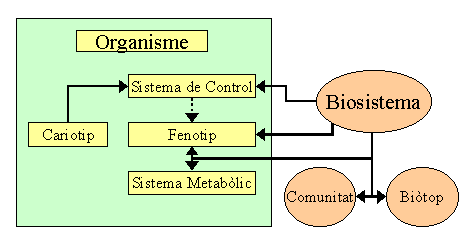
\includegraphics[width=6.1 in, keepaspectratio]{execucio}
	\fbox{\pdfimage{execucio.png}}
	\caption{Model d'execuci� d'instrucci�ns}
	\label{fig:execucioInstruccions}
\end{figure}

A grans trets, el funcionament �s el seg�ent:
\begin{enumerate}
\item Quan un organisme neix, es genera el sistema de control a partir del cariotip i s'inicialitzen de forma gen�rica el fenotip i el sistema metab�lic.
\item Un cop introdu�t l'organisme dins de la comunitat, el biosistema pot demanar-li instruccions al sistema de control.
\item El sistema de control consulta el fenotip i decideix quina instrucci� cal executar.
\item El sistema de control retorna al biosistema la instrucci� en q�esti�.
\item El biosistema completa la instrucci� amb par�metres que es troben dins del fenotip.
\item El biosistema executa la instrucci�. L'execuci� pot comportar consultes i/o modificacions sobre l'estat de:
\begin{itemize}
\item La comunitat i el bi�top
\item El fenotip i el sistema metab�lic del propi organisme.
\end{itemize}
\end{enumerate}


%%%%%%%%%%%%%%%%%%%%%%%%%%%%%%%%%%%%%%%%%%%%%%%%%%%%%%%%%%%%%%%%%%%%%
\subsection{Model metab�lic dels organismes}
%%%%%%%%%%%%%%%%%%%%%%%%%%%%%%%%%%%%%%%%%%%%%%%%%%%%%%%%%%%%%%%%%%%%%

\begin{figure}[ht]
\centering
\begin{tabular}{@{\extracolsep{.1 cm}}c@{\extracolsep{.1 cm}}c@{\extracolsep{.1 cm}}c@{\extracolsep{.1 cm}}c@{\extracolsep{-.1 cm}}c@{\extracolsep{.1 cm}}c@{\extracolsep{.1 cm}}c@{\extracolsep{.1 cm}}c@{\extracolsep{.1 cm}}}
    \begin{tabular}{|c|}
    \hline Medi\\ \hline
    \end{tabular}
    &
    \begin{tabular}{c}
        \\ excreci�
        \\ $\leftarrow$
        \\ $\rightarrow$
        \\ ingesti�
    \end{tabular}
    &
    \begin{tabular}{|c|}
    \hline Enmagatzem\\ de nutrients\\ \hline
    \end{tabular}
    &
    \begin{tabular}{c}
        \\ productes
        \\ $\leftarrow$
        \\ $\rightarrow$
        \\ reactius
    \end{tabular}
    &
    \begin{tabular}{|c|}
    \hline Reaccions\\ metab�liques\\ \hline
    \end{tabular}
    &
    \begin{tabular}{c}
        \\ endot�rmiques
        \\ $\leftarrow$
        \\ $\rightarrow$
        \\ exot�rmiques
    \end{tabular}
    &
    \begin{tabular}{|c|}
    \hline Energia\\ �til\\ \hline
    \end{tabular}
    &
    \begin{tabular}{c}
        \\ disipaci�
        \\ $\rightarrow$
        \\ $\rightarrow$
        \\ funcions
        \\ vitals
    \end{tabular}
\end{tabular}
    \caption{Model metab�lic dels organismes a Bioscena}
    \label{fig:modelMetabolic}
\end{figure}

Dintre de l'organisme hi ha dos formes de tenir l'energia:
\begin{itemize}
\item En forma d'energia �til.
\item En forma de nutrients.
\end{itemize}

No podem passar d'una a l'altre, si no �s mitjan�ant un proc�s
metab�lic. Per un costat, l'energia �til �s l'�nica que pot fer-se
servir a la majoria de processos vitals. Per un altre, aquesta
energia �til t� una caducitat de forma que, quan passa un cert temps
de la seva obtenci�, es disipa. La figura \ref{fig:modelMetabolic}
representa els cicles energ�tics dins d'un organisme.

%%%%%%%%%%%%%%%%%%%%%%%%%%%%%%%%%%%%%%%%%%%%%%%%%%%%%%%%%%%%%%%%%%%%%
\subsubsection{Fluxe de nutrients}
%%%%%%%%%%%%%%%%%%%%%%%%%%%%%%%%%%%%%%%%%%%%%%%%%%%%%%%%%%%%%%%%%%%%%

Com s'ha explicat a l'apartat \ref{sec:biotop}, els nutrients tenen
un identificador o patr� qualitatiu que indica quin tipus de nutrient
�s. Per seleccionar un nutrient dins d'un grup, nom�s cal oferir una
clau o patr� de cerca i una toler�ncia respecte a aquest patr�.
Cal recordar que la funci� de compatibilitat entre claus no �s 
determinista (apartat \ref{sec:compatibilitat}) i l'execuci� d'una 
mateixa cerca pot donar resultats diferents.

Un organisme pot introduir un nutrient en el seu cos des del medi
per ingesti� o des d'un altre organisme en atacar-lo.
An�logament, els nutrients es poden extreure del cos cap al medi 
per excreci� i cap un altre organisme en rebre un atac.

El nombre de nutrients que hi caben al pap d'un organisme pot estar 
limitat per configuraci�. De fet es recomana, donat que alguns 
organismes tendeixen a acomular-ne i se'n deriva un alt consum de
mem�ria. Al igual que succeeix al substrat, quan es sobrepassa el
l�mit, els nutrients m�s antics s'eliminen.

Per fer una reacci� metab�lica, s'extreuen els nutrients reactius 
del pap de l'organisme. D'aquesta reacci� s'obte un balan� d'energia
i uns productes que son introdu�ts al pap novament.


%%%%%%%%%%%%%%%%%%%%%%%%%%%%%%%%%%%%%%%%%%%%%%%%%%%%%%%%%%%%%%%%%%%%%
\subsubsection{Fluxe d'energia �til}
%%%%%%%%%%%%%%%%%%%%%%%%%%%%%%%%%%%%%%%%%%%%%%%%%%%%%%%%%%%%%%%%%%%%%

Segons els reactius, les reaccions metab�liques acaben sent ex�genes
o end�genes, �s a dir, proudeixen energia o en consumeixen.

El m�s normal segons el model �s obtindre energia �til a partir de 
les reaccions metab�liques ex�genes. Per�, �s possible configurar el 
biosistema per que certes accions, com el simple fet d'ingerir un 
nutrient, en generin energia �til. No dependre del metabolisme per 
obtindre energia permet implementar sistemes m�s simples, que 
facilitin la feina als organismes per sobreviure.

L'energia �til es consumeix per tres motius:
\begin{itemize}
\item Les contribucions energ�tiques a reaccions end�genes
\item El cost de les accions realitzades
\item La disipaci�
\end{itemize}

Es pot configurar el cost associat a cada funci� vital. Equilibrar
els costos i guanys energ�tics de les diferents operacions �s crucial 
per obtindre comportaments complexos en els organismes. Cal for�ar-los
a que desenvolupin estrat�gies complexes i que tinguin flexibilitat
de maniobra per evolucionar estrategies no �ptimes. 

La disipaci� de l'energia s'implementa amb un seguit de contenidors
cadascun dels quals t� una caducitat. L'energia obtinguda es fica en
el contenidor m�s nou, mentres que l'energia que perdem l'extreiem
dels contenidors m�s vells. Quan el contenidor m�s vell caduca,
l'energia que hi cont� es perd (es disipa) i s'afegeix un contenidor
nou buit. 

\begin{figure}[ht]
\centering
%    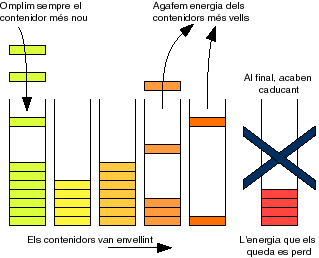
\includegraphics[width=6.1 in, keepaspectratio, draft]{disipacio}
    \fbox{\pdfimage{disipacio.png}}
    \caption{Disipaci� de l'energia obtinguda per l'organisme}
    \label{fig:disipacio}
\end{figure}



%%%%%%%%%%%%%%%%%%%%%%%%%%%%%%%%%%%%%%%%%%%%%%%%%%%%%%%%%%%%%%%%%%%%%
\subsection{Sist�ma d'her�ncia}
%%%%%%%%%%%%%%%%%%%%%%%%%%%%%%%%%%%%%%%%%%%%%%%%%%%%%%%%%%%%%%%%%%%%%

%%%%%%%%%%%%%%%%%%%%%%%%%%%%%%%%%%%%%%%%%%%%%%%%%%%%%%%%%%%%%%%%%%%%%
\subsubsection{Trets generals}
%%%%%%%%%%%%%%%%%%%%%%%%%%%%%%%%%%%%%%%%%%%%%%%%%%%%%%%%%%%%%%%%%%%%%

En aquest projecte, estan diferenciats els conceptes de cariotip i
genotip. El cariotip, simplement �s un seguit de dades, 
significatives o no, organitzades en cromosomes. El genotip �s la
interpretaci� de la informaci� �til que s'hi troba al cariotip i est�
organitzada en gens i que en el nostre cas serveix com a sistema de
control com s'explica m�s endavant.

Si els cromosomes que formen el cariotip s�n unitats estructurals del
material gen�tic, els gens que formen el genotip en s�n les seves 
unitats funcionals. 

Aquest diferenciaci� es justifica perqu�:
\begin{enumerate}
\item Permet un model multicromos�mic, amb un nombre i longitud de
cromosomes variable que possibilita solucions creatives 
\cite{VarLengthKargupta}.
\item Permet implementar, sobre els cromosomes, operadors de
mutaci� i creuament planers.
\item La traducci� de cariotip a genotip, ens permet detectar
promotors i terminadors \cite{ptGAs}, proporcionar operadors, 
eliminar introns \cite{IntronExonFoster}... Facilita d'aquesta 
forma la implementaci� d'aquests fen�mens.
\item �s m�s semblant al comportament biol�gic.
\end{enumerate}

%%%%%%%%%%%%%%%%%%%%%%%%%%%%%%%%%%%%%%%%%%%%%%%%%%%%%%%%%%%%%%%%%%%%%
\subsubsection{El cariotip i els cromosomes}
%%%%%%%%%%%%%%%%%%%%%%%%%%%%%%%%%%%%%%%%%%%%%%%%%%%%%%%%%%%%%%%%%%%%%

Cada organisme cont� un nombre variable de {\bf
cromosomes}\index{cromosoma!segons aquest projecte} que, en conjunt,
formen el {\bf cariotip}\index{cariotip!segons aquest projecte}. Cada
cromosoma est� format per una seq��ncia de bases representada
cadascuna amb un bit o un grup de bits.

Tot i que la unitat b�sica del cromosoma �s la base (un conjunt
redu�t de bits), a la implementaci�, no es considera aquesta unitat
m�s que per a fer algun tipus de mutaci� puntual. Per a la resta de
manipulacions ho farem a nivell de cod�, donat que no fa falta
arribar a nivell de base i �s m�s �ptim accedir-hi. En aquesta
representaci�, un cod� coincideix amb una paraula doble (32 bits).

El cromosoma, com a tal, no �s una unitat d'informaci� sin� un medi
on estan les dades gen�tiques. �s un medi que pot tenir errors i
provocar mutacions. Dins d'un organisme, la tasa de mutaci� de cada
cromosoma �s proporcional a la seva longitud.

%%%%%%%%%%%%%%%%%%%%%%%%%%%%%%%%%%%%%%%%%%%%%%%%%%%%%%%%%%%%%%%%%%%%%
\subsubsection{Mutacions}
%%%%%%%%%%%%%%%%%%%%%%%%%%%%%%%%%%%%%%%%%%%%%%%%%%%%%%%%%%%%%%%%%%%%%

El cariotip �s el responsable de les mutacions que passaran a la
descend�ncia (mutacions germinals, veure la p�gina \pageref{mutacioMolecular}).

% TODO: Ei, que al final no evoluciones la mutaci�

Tot i que la probabilitat de mutaci� ha de dependre, en gran mesura,
dels agents mut�gens del medi, els organismes han de poder controlar
gen�ticament la probabilitat de mutaci� per adaptar-la a la seva
situaci�. En posar en mans de l'evoluci� la probabilitat de mutar
estem confiant en que l'coevoluci� castigar� els organismes que no
mutin en front dels que mutin doncs els primers no podran millorar.

El control sobre la probabilitat de mutaci� d'un organisme es fa amb
una clau que t� el propi organisme. Aquesta clau es pot adaptar, en
major o menor mesura, al llarg del proc�s evolutiu, a una
d'equivalent que hi ha a cada posici� del substrat.

% TODO: Cal clarificar m�s com determinar la probabilitat de mutaci�.

Un cop es d�na, a un organisme, la probabilitat de mutar, cal decidir
com es fa la mutaci�, es a dir, amb quin operador de mutaci� es fa.
Cada organisme t� codificada gen�ticament una ponderaci� per a cada
operador de mutaci�.
\begin{equation}
  Probabilitat (operador_i) = {{ponderacio_i}\over\sum_j{ponderacio_j}}
  \label{eq:ponderacioOperadors}
\end{equation}

%% TODO: On es codifica la ponderaci� pels operadors de mutaci�

Els operadors de mutaci� s�n objectes que podem aplicar a un cariotip
per aplicar la mutaci�. Els operadors de mutaci� implementats es basen
en el funcionalment de les mutacions naturals i es divideixen en tres
categories segons el seu abast:
\begin{itemize}
\item {\em Mutaci� Cariot�pica:} Modifica el cariotip.
\begin{itemize}
\item {\em Mutaci� per fusi�:} Fusiona dos cromosomes.
\item {\em Mutaci� per escisi�:} Parteix en dos un cromosoma.
\item {\em Euploidia positiva:} Duplicaci� total del cariotip.
\item {\em Aneuploidia positiva:} Duplicaci� d'un cromosoma.
\item {\em Aneuploidia negativa:} Eliminaci� d'un cromosoma.
\end{itemize}
\item {\em Mutacio cromos�mica o estructural:} Modifica l'estructura 
d'un cromosoma. 
\begin{itemize}
\item {\em Mutaci� per delecci�:} Elimina un fragment del cromosoma.
\item {\em Mutaci� per despla�ament:} Despla�a un fragment de lloc 
dins del cromosoma.
\item {\em Mutaci� per inserci� aleat�ria:} Insereix al cromosoma un 
fragment aleatori.
\item {\em Mutaci� per inserci� replicada:} Insereix al cromosoma un 
fragment replicat del mateix cromosoma.
\end{itemize}
\item {\em Mutaci� g�nica o puntual:} Modifica el contingut d'una 
base o conjunt de bases.
\begin{itemize}
\item {\em Mutaci� puntual dr�stica:} Canvia una paraula (cod�) per un altre.
\item {\em Mutaci� puntual bin�ria:} Inverteix una base (bit) per un altre.
\item {\em Mutaci� puntual bin�ria en distribuci� gaussiana:} Inverteix aproximadament 4 bits d'un cod� (el nombre de bases modificades seg�eix una distribuci� normal).
\end{itemize}
\end{itemize}

%%%%%%%%%%%%%%%%%%%%%%%%%%%%%%%%%%%%%%%%%%%%%%%%%%%%%%%%%%%%%%%%%%%%%
\subsection{El sistema de control}
%%%%%%%%%%%%%%%%%%%%%%%%%%%%%%%%%%%%%%%%%%%%%%%%%%%%%%%%%%%%%%%%%%%%%

%%%%%%%%%%%%%%%%%%%%%%%%%%%%%%%%%%%%%%%%%%%%%%%%%%%%%%%%%%%%%%%%%%%%%
\subsubsection{Trets generals}
%%%%%%%%%%%%%%%%%%%%%%%%%%%%%%%%%%%%%%%%%%%%%%%%%%%%%%%%%%%%%%%%%%%%%

Per a la resta del sistema, la implementaci� interna del sistema de 
control �s indiferent. Podria ser una Xarxa neuronal com als LEE, 
per�, a l'exemple que es proposava aqu�, es pretenia comprovar si els 
mecanismes d'expressi� g�nica naturals poden ocupar aquest lloc.

El nostre sistema de control ha de simular aquests mecanismes.

%%%%%%%%%%%%%%%%%%%%%%%%%%%%%%%%%%%%%%%%%%%%%%%%%%%%%%%%%%%%%%%%%%%%%
\subsubsection{Els gens i el genotip}
%%%%%%%%%%%%%%%%%%%%%%%%%%%%%%%%%%%%%%%%%%%%%%%%%%%%%%%%%%%%%%%%%%%%%

El {\bf genotip}\index{genotip!segons aquest projecte} �s la
traducci� del cariotip a elements significatius. Aquests elements
significatius s'agrupen en {\bf gens}\index{gen!segons aquest
projecte}, que s'interpreten a partir dels codons del cromosoma.

Cada gen t� una zona operadora\index{zona operadora} que activa o
desactiva el gen segons certa condici� que ha de complir el fenotip o
indirectament, mitjan�ant el fenotip, del m�n exterior.

La zona estructural (seguint de forma aproximada la nomenclatura de
Jacob i Monod) �s la que es veu controlada per la zona operadora. 
Dins d'ella est� la informaci� (instruccions) que s'executar� si la 
zona operadora ho permet.

En resum, la transcripci� del cromosoma en gens constar� de diverses
parts:
\begin{enumerate}
\item Indentificaci� de la zona promotora (indica l'inici d'un
locus)
\item Indentificaci� de la zona terminadora corresponent (indica
el final d'un locus)
\item Identificaci� (justament despr�s de la zona promotora) i
interpretaci� de la zona operadora (indicar� quan cal executar el gen
tradu�t).
\item Eliminaci� d'introns (sequencies de codons no significatius) entre
promotora i terminadora (proc�s de maduraci�)
\item Traducci� de la zona estructural (la que porta les instruccions
que s'executaran amb el gen)
\end{enumerate}

Per raons d'optimitzaci�, la transcripci�, maduraci� i traducci� es 
fa nom�s una vegada durant la vida de l'organisme, encara que, a la 
natura, la transcripci� de l'ADN es fa cont�nuament. Aix� no t� 
implicacions massa importants, donat que ens guardem amb el gen el 
significat de la seva zona operadora que ens serveix per simular el 
comportament temporal de la transcripci�.


%%%%%%%%%%%%%%%%%%%%%%%%%%%%%%%%%%%%%%%%%%%%%%%%%%%%%%%%%%%%%%%%%%%%%
\subsection{El fenotip}
%%%%%%%%%%%%%%%%%%%%%%%%%%%%%%%%%%%%%%%%%%%%%%%%%%%%%%%%%%%%%%%%%%%%%

El que anomenem pr�piament {\em fenotip}\index{fenotip!segons aquest
projecte} �s un conjunt de 16 registres de 32 bits que t� cada
organisme. Representen el cos f�sic de l'organisme.

El fenotip es modifica per acci� directa del genotip. Sovint, si es
tracta d'operacions sensorials, aquestes modificacions depenen del
medi o de l'estat intern. Les operacions tamb� poden ser motores, i
en aquest cas el contingut del fenotip �s qui afecta el medi i/o 
l'estat intern modificant les instruccions expedides per l'organisme. 

Per �ltim, cal remarcar que el fenotip �s un dels dos mitjans que
t�nen els organismes per recon�ixer els altres, juntament amb la 
detecci� de mol�l�cules excretades. Hi ha instruccions sensores el 
resultat de les quals dep�n del fenotip de l'organisme que es troba 
a una posici� relativa.

En resum, el fenotip �s el mecanisme principal d'interacci� que tenen
els organismes.


%%%%%%%%%%%%%%%%%%%%%%%%%%%%%%%%%%%%%%%%%%%%%%%%%%%%%%%%%%%%%%%%%%%%%
\newpage


%%%%%%%%%%%%%%%%%%%%%%%%%%%%%%%%%%%%%%%%%%%%%%%%%%%%%%%%%%%%%%%%%%%%%
%
%

%%%%%%%%%%%%%%%%%%%%%%%%%%%%%%%%%%%%%%%%%%%%%%%%%%%%%%%%%%%%%%%%%%%%%
\chapter{Mecanismes d'especiaci� i an�lisi}
%%%%%%%%%%%%%%%%%%%%%%%%%%%%%%%%%%%%%%%%%%%%%%%%%%%%%%%%%%%%%%%%%%%%%

%%%%%%%%%%%%%%%%%%%%%%%%%%%%%%%%%%%%%%%%%%%%%%%%%%%%%%%%%%%%%%%%%%%%%
\section{Els taxonomistes}
%%%%%%%%%%%%%%%%%%%%%%%%%%%%%%%%%%%%%%%%%%%%%%%%%%%%%%%%%%%%%%%%%%%%%

\index{taxonomista}
\index{grup reproductiu}
\index{esp�cie|see{grup reproductiu}}
Per que l'usuari pugui extreure una informaci� �til, cal que poguem
agrupar els organismes en esp�cies. �s clar que a la nostra comunitat,
al igual que a la natura, l'especiaci� �s un fen�men que cal que
emergeixi, L'esp�cie, no �s quelcom intr�nsec a tot organisme; �s a
dir, que el concepte d'esp�cie no estar� implementat al codi gen�tic
o als mecanismes de funcionament comuns dels organismes sin� que
caldr� observar-ho en el seu comportament.

Els taxonomistes s�n objectes que agrupen organismes per afinitat
evolutiva segons els conceptes abans mencionats.

Com que, abans de definir objectius, em plantejava implementar
organismes amb reproducci� sexual, vaig construir un taxonomista que
soportava tota la complexitat que comporten els creuaments i que he
mencionat abans.

Com finalment, els intercanvis sexuals es van excloure dels objectius 
del projecte, les relacions evolutives es limiten a un arbre i vaig 
implementar un taxonomista molt m�s senzill, que simplement discrimina 
organismes amb diferent cromosoma quan es produeix una mutaci�, per�, 
que compleix el mateix protocol que el m�s elaborat implementat 
anteriorment de forma que es podrien intercanviar.

El taxonomista simple �s el que he fet servir a les proves donat que
era molt m�s r�pid i la informaci� que dona ja �s suficient per la
complexitat dels sistemes generats. 

Tot i aix�, documento el taxonomista per organismes sexuals de cara 
a ilustrar millor el protocol i donat que ser� �til en futures 
ampliacions del sistema si s'afegeixen creuaments.

%%%%%%%%%%%%%%%%%%%%%%%%%%%%%%%%%%%%%%%%%%%%%%%%%%%%%%%%%%%%%%%%%%%%%
\section{Qu� es vol solucionar}
%%%%%%%%%%%%%%%%%%%%%%%%%%%%%%%%%%%%%%%%%%%%%%%%%%%%%%%%%%%%%%%%%%%%%

El concepte cl�ssic d'esp�cie considera que dos organismes s�n de la
mateixa esp�cie si s�n capa�os de donar descenc�ncia f�rtil.

A la biologia moderna es considera que la diferenciaci� de les esp�cies
no est� tant en la capacitat sin� en el fet mateix de reproduir-se.
En aix� pot influir:
\begin{itemize}
\item   Compatibilitat gen�tica
\item   Compatibilitat d'acoplament
\item   Compatibilitat geogr�fica
\item   Altres
\end{itemize}

Tamb�, cal adonar-se de que totes aquestes consideracions es
refereixen als organismes que es reprodueixen sexualment i es creuen.
C�m es poden identificar les esp�cies dels organismes que es
reprodueixen asexualment (com �s el cas implementat)? En quin punt es 
considera que dos descendents d'un mateix organisme s�n d'una 
esp�cie diferent?

A m�s, degut a la seva qualitat emergent, l'especiaci� no estar�
sempre ben definida. Tamb� pot ser que la selecci� a l'hora de
reproduir-se tingui en compte altres mecanismes que no pas
l'especiaci�.

Tota aquesta conjuntura ha obligat a deixar de banda el concepte
d'esp�cie cap al concepte, una mica m�s relaxat, de grup reproductiu
que, tot i la relaxaci�, segueix proporcionant informaci� �til sobre
les diferents poblacions del biosistema. Considerem que un grup
reproductiu �s un conjunt d'organismes que es creuen entre s� o
provenen d'ancestres comuns o ancestres que s'han creuat entre s� 
dintre d'un cert per�ode de temps o d'un cert nombre de generacions.

%%%%%%%%%%%%%%%%%%%%%%%%%%%%%%%%%%%%%%%%%%%%%%%%%%%%%%%%%%%%%%%%%%%%%
\subsection{Taxonomista d'organismes sexuals}
%%%%%%%%%%%%%%%%%%%%%%%%%%%%%%%%%%%%%%%%%%%%%%%%%%%%%%%%%%%%%%%%%%%%%

\index{taxonomista!amb sexualitat}
La pol�tica que determina els grups reproductius es basa en un marcatge
hist�ric.

Cada individu s'associa amb un tax� que no �s m�s que una seq��ncia de
marques amb diferent antiguitat. Les marques es traspasen id�ntiques a
la descend�ncia via mitosi.

Cada cert temps, es fa una discriminaci� que consisteix en fondre les
dos marques m�s antigues de cada tax� en una sola i afegir una marca
nova que diferenciar� els individus que fins llavors compartien les
mateixes marques i que pendr� import�ncia a mida que adquireixi antiguitat.

C�m es produir� aquesta discriminaci�? Imaginem que existeixen individus
amb els taxons seg�ents:
\begin{center}
\begin{tabular}{p{45 mm}cp{45 mm}cp{45 mm}}
\begin{center}
\begin{tabular}{l}
A A A A A A\\
A A A A A A\\
A B A A A A\\
A B B A A A\\
A B B A A A\\
B A A A A A
\end{tabular}
\end{center}
&&
\begin{center}
\begin{tabular}{l}
{\bf A} A A A A\\
{\bf A} A A A A\\
{\bf B} A A A A\\
{\bf B} B A A A\\
{\bf B} B A A A\\
{\bf C} A A A A
\end{tabular}
\end{center}
&&
\begin{center}
\begin{tabular}{l}
A A A A A {\bf A}\\
A A A A A {\bf B}\\
B A A A A {\bf A}\\
B B A A A {\bf A}\\
B B A A A {\bf B}\\
C A A A A {\bf A}
\end{tabular}
\end{center}
\\Taxons originals dels organismes abans de la discretitzaci� de la poblaci�
&$\Rightarrow$
&Fusi� dels dos taxons m�s antics
&$\Rightarrow$
&Discriminaci� dels individus amb les mateixes marques amb una nova:
\end{tabular}
\end{center}

D'altra banda, hem de considerar el que passa quan es creuen dos
individus que pertanyen a diferents taxons.

Quan dos individus es creuen, s'asimilen les marques des de la marca
m�s antiga fins a la primera que els diferencia als dos (marca discriminant). Es a dir, a tots els taxons cal revisar les marques. Pot ser es veu m�s clar amb un exemple. Considerem el seg�ent conjunt de taxons.

\begin{tabular}{l}
A A A A A A\\
A A A A A B\\
A A A A B B\\
A A A B A B\\
A A A B B A\\
A A A B B B\\
A A B A A A
\end{tabular}

Si es creuen AAAABB i AAABBA, cal considerar equivalemts les
subseq�encies de marques AAAA i AAAB equivalents.
Tots els taxons que comencin per AAAB els canviem per AAAA sense
oblidar-nos de modificar la seg�ent marca m�s jove que la discriminant
amb l'objectiu de que els taxons asimilats mantinguin el sentit.

\begin{tabular}{lcl}
A A A A A A&$\dashrightarrow$&A A A A A A\\
A A A A A B&$\dashrightarrow$&A A A A A B\\
A A A A B B&$\dashrightarrow$&A A A A B B\\
A A A B A B&$\Rightarrow$&A A A {\em A C} B\\
A A A B B A&$\Rightarrow$&A A A {\em A D} A\\
A A A B B B&$\Rightarrow$&A A A {\em A D} B\\
A A B A A A&$\dashrightarrow$&A A B A A A
\end{tabular}

De cara a la implementaci�, he considerat separar la major part
del proc�s associat a la determinaci� de grups reproductius en
un objecte independent anomenat taxonomista. Aquest objecte s'encarrega de mantenir els taxons al dia mitjan�ant una interf�cie estreta que mant� amb el processador.

A dins de la comunitat es mant� una informaci� m�nima: l'identificador del tax� al que pertany cada individu. El tr�fec d'informaci� a l'exterior del objecte taxonomista es basa exclusivament en el pas d'aquests identificadors. La interf�cie oferida permet al processador:

\begin{itemize}
\item   Incrementar o decrementar la poblacio assignada a un tax�
\item   Creuar un parell de taxons
\item   Generar un nou tax� (Per individus generats espont�niament)
\item   Envellir les marques i discriminar la poblaci� que comparteix el mateix tax�
\item   Determinar el grau de parentesc entre dos individus
\end{itemize}

Quan hem de discriminar o quan fussionem dos taxons, necessitem
que la Comunitat i el Taxonomista cooperin.

Quan cal discriminar la poblaci�, la Comunitat demana al Taxonomista,
per a cada individu, un nou tax�, basant-se en el tax� antic i el
n�mero de individus que en queden sense discriminar d'aquest.

El nou taxo duu les marques X.X.X. ... .X.N on N �s el n�mero de
queden sense discriminar.

Quan, fruit d'un creuament, es fusionen dos taxons, un dels dos
taxons �s assimilat per l'altre i, en conseq��ncia, els individus
associats al tax� assimilat, cal associar-los al tax� assimilador.

Per dins, el taxonomista est� compost per una llista indexada de
taxons (taxonari). Els n�meros d'�ndex es referencien des de cada
individu pertanyent a la Comunitat.

Una alternativa al taxonari hagu�s sigut una implementaci� en arbre
en comptes de la llista indexada. En cada node hi hauria una marca
i a les fulles els identificadors de cada tax�. La implementaci� en
arbre simplifica molt la l�gica dels algorismes de discriminaci� i
creuament per� complica altres operacions internes que amb la llista
indexada s�n trivials.

La llista indexada permet un acc�s directe als taxons i, a m�s, els
mant� ordenats de tal forma que les cerques de grups de parentesc
tenen un cost temporal m�nim.



%%%%%%%%%%%%%%%%%%%%%%%%%%%%%%%%%%%%%%%%%%%%%%%%%%%%%%%%%%%%%%%%%%%%%
\newpage

% Time Log
%

%%%%%%%%%%%%%%%%%%%%%%%%%%%%%%%%%%%%%%%%%%%%%%%%%%%%%%%%%%%%%%%%%%%%%%
\chapter{Manual del programador}
%%%%%%%%%%%%%%%%%%%%%%%%%%%%%%%%%%%%%%%%%%%%%%%%%%%%%%%%%%%%%%%%%%%%%%

%%%%%%%%%%%%%%%%%%%%%%%%%%%%%%%%%%%%%%%%%%%%%%%%%%%%%%%%%%%%%%%%%%%%%%
\section{Compilaci�}
%%%%%%%%%%%%%%%%%%%%%%%%%%%%%%%%%%%%%%%%%%%%%%%%%%%%%%%%%%%%%%%%%%%%%%

%%%%%%%%%%%%%%%%%%%%%%%%%%%%%%%%%%%%%%%%%%%%%%%%%%%%%%%%%%%%%%%%%%%%%%
\subsection{Generaci� de n�meros de compilaci�}
%%%%%%%%%%%%%%%%%%%%%%%%%%%%%%%%%%%%%%%%%%%%%%%%%%%%%%%%%%%%%%%%%%%%%%

Per generar n�meros de compilaci�, cal el programa {\tt buildnum},
el codi font del qual est� disponible a la pagina 
\begin{verbatim}
http:\\www.salleurl.edu\~is04069\Codders
\end{verbatim}

Si no es vol fer servir aquest programa, cal treure les crides que 
s'hi fan al {\tt makefile} o als fitxers de projecte.

%%%%%%%%%%%%%%%%%%%%%%%%%%%%%%%%%%%%%%%%%%%%%%%%%%%%%%%%%%%%%%%%%%%%%%
\subsection{GCC/DJGPP}
%%%%%%%%%%%%%%%%%%%%%%%%%%%%%%%%%%%%%%%%%%%%%%%%%%%%%%%%%%%%%%%%%%%%%%

Aquest compilador i, sobretot, la seva versi� per a DOS, el DJGPP, ha 
sigut el m�s testejat. De cara a compilar cal una versi� superior a la 
TODO i, per fer-ho sense problemes cal la TODO.

Per aquest compilador, es proveeix un fitxer {\tt makefile}. Cal 
assegurar-se que estan instalades les llibreries de 

El procediment �s el seg�ent:
\begin{enumerate}
\item Adaptar les variables seg�ents variables del makefile als noms
dels executables al sistema on es compila:
\begin{description}
\item [CC] Nom del compilador de C. ({\tt gcc}, {\tt cc}, {\tt egcs}...)
\item [CPPC] Nom del compilador C++. ({\tt c++}, {\tt cxx}...)
\item [RM] Comanda per esborrar arxius
\item [EXEC] Nom del executable generat
\end{description}
\item Si cal, comenta les crides a 'buildnum' que es fan als makefiles
\item Si es vol optimitzar per una maquina en concret, cal afegir '-march=ix86' a la variable CFLAGS del makefile; on x={3,4,5,6}
\item Escriure- 'make' i ale.
\end{enumerate}

Posibles problemes:
\begin{itemize}
\item Si teniu una versi� del compilador inferior a la TODO, dona 
problemes a la linia 170 de Cariotip.cpp.
A sota de la mateixa linia hi ha un fragment de codi substitutori
per a la l�nia del error, amb indicacions de com arreglar-ho.
\end{itemize}

%%%%%%%%%%%%%%%%%%%%%%%%%%%%%%%%%%%%%%%%%%%%%%%%%%%%%%%%%%%%%%%%%%%%%%
\subsubsection{Problemes en sistemes UNIX (Linux)}
%%%%%%%%%%%%%%%%%%%%%%%%%%%%%%%%%%%%%%%%%%%%%%%%%%%%%%%%%%%%%%%%%%%%%%

Els arxius de text del comprimit estan en format MS-DOS. Per aix�, cal 
treure els salts de carro adicional que impideixen la compilaci�.

La forma m�s r�pida de fer-ho �s fer servir l'opci� {\tt -a} quan es
descomprimeix el comprimit amb la utilitat {\tt unzip}.

%%%%%%%%%%%%%%%%%%%%%%%%%%%%%%%%%%%%%%%%%%%%%%%%%%%%%%%%%%%%%%%%%%%%%%
\subsection{Microsoft Visual C++}
%%%%%%%%%%%%%%%%%%%%%%%%%%%%%%%%%%%%%%%%%%%%%%%%%%%%%%%%%%%%%%%%%%%%%%

Dins de l'arxiu comprimit hi ha un projecte per Microsoft Visual C++
anomenat {\tt Bioscena.dsw}.

%%%%%%%%%%%%%%%%%%%%%%%%%%%%%%%%%%%%%%%%%%%%%%%%%%%%%%%%%%%%%%%%%%%%%%
\subsubsection{Problemes amb versions antigues}
%%%%%%%%%%%%%%%%%%%%%%%%%%%%%%%%%%%%%%%%%%%%%%%%%%%%%%%%%%%%%%%%%%%%%%

Amb versions antigues del compilador (TODO) es donen un parell de problemes:

\begin{itemize}
\item
Hi ha problemes amb la biblioteca est�ndard C++ que proporciona 
l'entorn degut a conflictes entre la implementaci� dels templates que 
fa el compilador i la forma de fer-los servir en la biblioteca, 
implementada per HP.
Es pot compilar l'eina si es modifiquen els fonts de la biblioteca, 
ficant entre comentaris les funcions que donen errors.
\item
No suporten massa b� punters a funcions membres.
El codi que fa servir punters a funcions membres, tot i que compila, 
genera un assembler no massa correcte i d�na errors d'execuci�.
\end{itemize}

%%%%%%%%%%%%%%%%%%%%%%%%%%%%%%%%%%%%%%%%%%%%%%%%%%%%%%%%%%%%%%%%%%%%%%
\subsection{Compilant amb altres compiladors}
%%%%%%%%%%%%%%%%%%%%%%%%%%%%%%%%%%%%%%%%%%%%%%%%%%%%%%%%%%%%%%%%%%%%%%

Per compilar amb altres compiladors, es requereix com a m�nim un 
compilador que suporti templates i punters a funcions membres i que
tingui implementada de forma suficientment amplia la llibreria 
est�ndar C++ segons s'especifica en l'est�ndard ISO/ANSI \ref{TODO}. 
Concretament es fan servir les cap�aleres est�ndard 
{\tt <algorithm>}, {\tt <functional>}, 
{\tt <list>}, {\tt <vector>}, {\tt <map>}, {\tt <deque>}, {\tt <string>}, 
{\tt <iostream>}, {\tt <fstream>}, {\tt <iomanip>} i {\tt <strstream>}.

%%%%%%%%%%%%%%%%%%%%%%%%%%%%%%%%%%%%%%%%%%%%%%%%%%%%%%%%%%%%%%%%%%%%%%
\section{Programaci� de noves topologies per els bi�tops}
%%%%%%%%%%%%%%%%%%%%%%%%%%%%%%%%%%%%%%%%%%%%%%%%%%%%%%%%%%%%%%%%%%%%%%

Si l'usuari necessit�s crear un nou tipus de topologia, cal que la
faci heretar de CTopologia, que �s la classe que defineix el m�nim per
reservar memoria pel substrat de cada posici�. CTopologia tamb�
estableix el protocol que han de seguir les subclasses, perqu� la
resta del sistema l'acepti sense haver de canviar-ho.

El secret est� en el fet de que tot el sistema manega identificadors
de posicions que s�n enters sense signe de 32 bits. Tot el significat
que poden tenir aquests identificadors el manega la topologia
internament.

Quan es deriva de CTopologia, el principal que caldria redefinir,
si cal, �s:
\begin{itemize}
\item   Un {\bf constructor} significatiu per a la topologia. Per exemple, en
    una topologia rectangular �s significatiu indicar l'altura i l'amplada.
    El constructor de CTopologia simplement reserva espai per N casselles.
    Caldria calcular aquesta N per passar-se-la.
\item   {\tt t\_posicio CTopologia::desplacament (t\_posicio origen, t\_desplacament desplacament)}:
    Una funci� per averiguar la posici� dest� en aplicar-li un vector
    de despla�ament a una posici� origen.
    CTopologia, la defineix de tal forma que el resultat �s una posici�
    dest� aleat�ria.
\item   {\tt bool CTopologia::esValid(t\_posicio id)}:
    Una funci� per saber si un identificador �s v�lid. Nom�s cal
    redefinir-ho si es modifica la correspond�ncia directa entre
    identificador de posici� i index de cassella en l'array de
    substrats reservada per CTopologia::CTopologia
\item   {\tt t\_posicio CTopologia::posicioAleatoria ()}:
    Una funci� per obtindre aleat�riament una posici� v�lida de la
    topologia. La funci� general que no caldria redefinir seria
    \begin{verbatim}
        {
            uint32 pos;
            do {pos=rnd.get();} while (!esValid(pos));
            return pos
        }
    \end{verbatim}
    per�, CTopologia no fa servir aquest algorisme donat que
    optimitza agafant un n�mero aleatori entre 0 i N. Aquesta
    optimitzaci� funciona mentre es mantingui la correspond�ncia
    entre identificador i index abans comentada.
    Si la subclasse la trenca, es quan cal redefinir la funci�.
\item   {\tt bool CTopologia::unio (t\_posicio origen, t\_posicio desti, t\_desplacament \& desp)}:
    Una funci� per calcular el primer d'un conjunt de desplacaments
    que cal fer per anar de l'origen al dest�.
    Retorna cert si el desplacament �s suficient per arribar a la posici� dest�.
    CTopologia, la defineix de tal forma que el resultat �s un despla�ament
    aleatori i retorna sempre fals (mai hi arriba).
\end{itemize}

Pot ser molt ilustratiu, de cara a implementar noves topologies,
fixar-se en les ja existents com CTopologiaToroidal.

%%%%%%%%%%%%%%%%%%%%%%%%%%%%%%%%%%%%%%%%%%%%%%%%%%%%%%%%%%%%%%%%%%%%%%
\section{Programaci� de nous agents}
%%%%%%%%%%%%%%%%%%%%%%%%%%%%%%%%%%%%%%%%%%%%%%%%%%%%%%%%%%%%%%%%%%%%%%

De cara a afegir nous agents al sistema, s'aconsella seguir els
seg�ents passos:

\begin{enumerate}
\item
    Llegir per sobre el codi dels agents ja implementats per
    assimilar les solucions que s'han donat a problemes que
    segurament es tornaran a repetir als nous agents.
    Tamb� conv� mantenir uniforme l'estil de programaci� i
    l'ordre intern dels fitxers per fer-ho m�s mantenible
    a tercers.
    El m�s pr�ctic es partir d'una c�pia d'un agent que tingui,
    estructuralment, tot o gran part del que interesa implementar.
\item
    Escollir la classe d'agent de la que volem heretar l'agent.
    Generalment voldrem que el nou agent pertanyi a un dels quatre
    grans grups funcionals d'agents:
    \begin{itemize}
    \item   Subordinadors (CMultiAgent i subclasses) si controla l'accionat d'altres agents
    \item   Posicionadors (CPosicionador i subclasses) si controla una posici� en el bi�top
    \item   Direccionadors (CDireccionador i subclasses) si controla una direcci�
    \item   Actuadors (CActuadors i subclasses) si modifica el substrat a una posici�
    \end{itemize}
    Si no pertany a cap dels quatre grups, caldria plantejar-se
    heretar de CAgent directament. En aquest cas, conv� fer un
    esfor� i fer una classe intermitja que pugui englobar altres
    agents en el futur.
    Anomenarem CAgentNou al nou agent afegit i CAgentVell a l'agent
    del qual heretem.
\item
    Adaptar el constructor de CAgentNou per que proveeixi els
    par�metres del constructor de la superclasse.
    Posicionadors i direccionadors, per exemple, necessiten una
    refer�ncia a un bi�top en el constructor. A les classes
    derivades de CPosicionador est� implementat com fer-ho.
\item
    Afegir dins del constructor, la l�nia.
    \\{\tt m\_tipus+="/ElMeuSubtipus";}\\
    que afegeix la cadena de subtipus a l'identificador de tipus
    que hereta de la superclasse.
\item
    Afegir els nous atributs (variables membre) dels que en dep�n
    l'estat de l'agent i les funcions d'acc�s als mateixos.
\item
    Inicialitzar dins del constructor els nous atributs als
    valors per defecte.
    Els atributs que siguin depend�ncies amb altres agents,
    o agents subordinats, es recomana que siguin punters, i no
    refer�ncies, per poder-ho deixar sense especificar
    al constructor. S'inicialitzen sempre com a punter
    a NULL. Cal procurar que, si el punter no apunta a un
    agent v�lid el seu valor sigui NULL i tenir-ho en compte
    quan hi accedim per evitar accesos il�legals a mem�ria.
    Es veu clarament aquesta idea llegint el codi d'alguns
    agents que ho fan.
\item
    Afegir dins del destructor, l'alliberament de mem�ria ocupada
    pels agents subordinat. Les depend�ncies no s'han de alliberar
    pas.
\item
    Redefinir la funci� membre {\tt virtual void CAgentNou::operator() (void)}
    per que faci el que hagi de fer quan l'agent �s accionat.
    Si es tracta d'un actuador, no cal redefinir aquesta sino
    {\tt virtual void CAgentNou::operator() (CSubstrat \& s)} on
    {\tt s} �s el substrat que hem de modificar.
    \footnote{Veure l'apartat \ref{TODO} que parla del que cal fer si es redefineix el substrat}
\item
    Redefinir la funci� {\tt virtual void CAgentNou::dump(CMissatger \& msg)}
    per que cridi a la funci� corresponent de la superclasse
    (CAgentVell a l'exemple) i, despr�s, inserti en el CMissatger
    les noves l�nies de configuraci� dels par�metres que afegeix l'agent:
    \begin{verbatim}
    void CAgentNou::dump(CMissatger & msg)
    {
        CAgentVell::dump(msg);
        msg << "- UnParametreNou " << m_valor1 << " " << valor2 << endl;
        msg << "- UnAltreParametreNou " << m_valor3 << endl;
    }
    \end{verbatim}
\item
    Redefinir la funci� {\tt virtual bool CAgentNou::configura(string parametre, istream \& valors, t\_diccionariAgents \& diccionari, CMissatger \& errors)}
    per mirar si el {\tt parametre} �s un dels que ha afegit CAgentNou.
    Si ho �s cal parsejar l'istream {\tt valors} en busca dels valors
    corresponents, reportar els errors que es produeixin pel CMissatger
    {\tt errors} i retornar cert per dir que el par�metre era de la classe.
    Si no ho �s, cal cridar a la funci� corresponent de la superclasse
    per que ho pugui interceptar ella.
    El diccionari serveix per, donat un nom d'agent de l'arxiu,
    obtindre un punter a l'agent que s'ha creat que, pot ser, t�
    un nom diferent.
    El diccionari �s un {\tt map<string, CAgent*>}, el seu funcionament
    s'explica a qualsevol manual sobre les Standard Template
    Libraries de C++.
    La estructura general de la funci� configura quedar� com aix�:

    \begin{verbatim}
    bool CAgentNou::configura(string parametre, istream & valors,
    t_diccionariAgents & diccionari, CMissatger & errors)
    {
        if (parametre=="UnParametreNou") {
            // Parsing dels valors...
            return true;
        }
        if (parametre=="UnAltreParametreNou") {
            // Parsing dels valors...
            return true;
        }
        // Li deixem a la superclasse que l'intercepti si vol
        return CAgentVell::configura(parametre, valors, diccionari, errors);
    }
    \end{verbatim}
\item
    Si cap dels atributs (m\_dependencia a l'exemple) �s una
    depend�ncia amb altre agent, cal redefinir la seg�ent funci� com segueix:
    \begin{verbatim}
    list<CAgent*> CAgentNou::dependencies() {
        list<CAgent*> l=CAgentVell::dependencies();
        if (m_dependencia) l.push_back(m_dependencia);
        return l;
    }
    \end{verbatim}
\item
    Si cap dels atributs (m\_subordinat a l'exemple) �s un
    agent subordinat, cal redefinir la seg�ent funci� com segueix:
    \begin{verbatim}
    list<CAgent*> CAgentNou::subordinats() {
        list<CAgent*> l=CAgentVell::subordinats();
        if (m_subordinat) l.push_back(m_subordinat);
        return l;
    }
    \end{verbatim}
\item
    Afegir a l'arxiu {\tt Agent.cpp} un include a {\tt AgentNou.h}
    i, a la funci� est�tica CAgent::CreaAgent(...) una l�nia com
    les que ja n'hi ha per cada tipus d'agent, per�, per a CAgentNou.
    Aix� permet que la funci� CAgent::ParsejaArxiu pugui recon�ixer
    el nou tipus als arxius de configuraci�.

\end{enumerate}

De tots els punts anteriors el que potser �s una mica m�s
particularitzat s�n els atributs i els m�todes d'acc�s als mateixos,
i el m�tode d'accionament (o d'actuaci� en el cas dels actuadors).
Per a la resta de coses el m�s pr�ctic es fer un cut\&paste dels agents
ja implementats i retocar el m�nim.


%% TODO: Programaci� de nous substrats


%%%%%%%%%%%%%%%%%%%%%%%%%%%%%%%%%%%%%%%%%%%%%%%%%%%%%%%%%%%%%%%%%%%%%%

\appendix
%%%%%%%%%%%%%%%%%%%%%%%%%%%%%%%%%%%%%%%%%%%%%%%%%%%%%%%%%%%%%%%%%%%%%
%
%

\nocite{*} % Per que surti tot
\bibliographystyle{alpha}
\bibliography{bibliografia,bibliografia}

\label{TODO}
\printindex

%% TODO: Treure aixo dels links
%\hyperlink{kaja}{Origen}
%\hypertarget{kaja}{Desti}

\end{document}
